\documentclass{article}

% if you need to pass options to natbib, use, e.g.:
%     \PassOptionsToPackage{numbers, compress}{natbib}
% before loading neurips_2024


% ready for submission
% \usepackage{neurips_2024}

\usepackage[preprint]{neurips_2024}
\usepackage[english]{babel}

\usepackage{pythonhighlight}
\usepackage{wrapfig,lipsum}
\usepackage{algorithm}
%\usepackage{algorithmic}


\usepackage{amsmath, amssymb, amsfonts} % for math symbols
\usepackage{bm}                         % for \bm (bold math)
\usepackage{mathtools}                 % for \vect and improved math
\usepackage{bbm}                        % if you use \mathbbm

\usepackage{algpseudocode}
\usepackage{amsthm}
\usepackage{todonotes}
\usepackage{multirow}
\usepackage[colorlinks=true, allcolors=blue]{hyperref}
% Set page size and margins
% Replace `letterpaper' with `a4paper' for UK/EU standard size
%\usepackage[letterpaper,top=2cm,bottom=2cm,left=3cm,right=3cm,marginparwidth=1.75cm]{geometry}
% Useful packages
%\usepackage{amsthm,amsmath,amssymb}
%\usepackage{amsthm}
\usepackage{graphicx}
\usepackage[colorlinks=true, allcolors=blue]{hyperref}





% to compile a preprint version, e.g., for submission to arXiv, add add the
% [preprint] option:
%     \usepackage[preprint]{neurips_2024}


% to compile a camera-ready version, add the [final] option, e.g.:
%     \usepackage[final]{neurips_2024}


% to avoid loading the natbib package, add option nonatbib:
%    \usepackage[nonatbib]{neurips_2024}


\usepackage[utf8]{inputenc} % allow utf-8 input
\usepackage[T1]{fontenc}    % use 8-bit T1 fonts
\usepackage{hyperref}       % hyperlinks
\usepackage{url}            % simple URL typesetting
\usepackage{booktabs}       % professional-quality tables
\usepackage{amsfonts}       % blackboard math symbols
\usepackage{nicefrac}       % compact symbols for 1/2, etc.
\usepackage{microtype}      % microtypography
\usepackage{xcolor}         % colors
\usepackage{amsmath, amssymb}
\usepackage{natbib}
\usepackage{listings}

\newcommand{\hidesection}[1]{}

\DeclareMathOperator{\vect}{vec}

\newtheorem{theorem}{Theorem}

\lstset{
    language=Python,
    basicstyle=\ttfamily\small,
    keywordstyle=\color{blue},
    commentstyle=\color{gray},
    stringstyle=\color{red},
    numbers=left,
    numberstyle=\tiny\color{gray},
    stepnumber=1,
    numbersep=5pt,
    backgroundcolor=\color{white},
    showspaces=false,
    showstringspaces=false,
    showtabs=false,
    frame=single,
    tabsize=2,
    captionpos=b,
    breaklines=true,
    breakatwhitespace=false,
    escapeinside={\%*}{*)}
}


%\title{Fast Kronecker-Factored Fisher Approximation for Efficient LLMs Compression}
\title{Generalized Fisher-Weighted SVD: Scalable Kronecker-Factored Fisher Approximation for Compressing Large Language Models}


% The \author macro works with any number of authors. There are two commands
% used to separate the names and addresses of multiple authors: \And and \AND.
%
% Using \And between authors leaves it to LaTeX to determine where to break the
% lines. Using \AND forces a line break at that point. So, if LaTeX puts 3 of 4
% authors names on the first line, and the last on the second line, try using
% \AND instead of \And before the third author name.


\author{%
  Viktoriia Chekalina \\
  AIRI\\
  \texttt{Chekalina@airi.net} \\
  % examples of more authors
   \And
    Daniil Moskovskiy \\
   AIRI, Skoltech \\
   \texttt{Daniil.Moskovskiy@skoltech.ru} \\
   \AND
   Daria Cherniuk\\
   AIRI \\
   \And
   Maxim Kurkin \\
   AIRI, Skoltech \\
   \And
   Andrey Kuznetsov \\
   AIRI \\
   \And
   Evgeny Frolov \\
   AIRI, HSE University\\
}


\begin{document}


\maketitle


\begin{abstract}


The Fisher information is a fundamental concept for characterizing the sensitivity of parameters in neural networks. However, leveraging the full observed Fisher information is too expensive for large models, so most methods rely on simple diagonal approximations. While efficient, this approach ignores parameter correlations, often resulting in reduced performance on downstream tasks. In this work, we mitigate these limitations  and propose Generalized Fisher-Weighted SVD (GFWSVD) — a post-training LLM compression technique that accounts for both diagonal and off-diagonal elements of the Fisher information matrix, providing a more accurate reflection of parameter importance. To make the method tractable, we introduce a scalable adaptation of the Kronecker-factored approximation algorithm for the observed Fisher information. We demonstrate the effectiveness of our method on LLM compression, showing improvements over existing compression baselines.

\end{abstract}


\section{Introduction}

The Fisher information Fisher Information Matrix (FIM)~\cite{Fisher1992} is widely employed in neural networks to enhance the efficiency of models, particularly in the context of training and inference. However, computing and leveraging the full Fisher information is computationally prohibitive for deep networks. To make the problem tractable, existing methods adopt simplified approximations -- most commonly, assuming that the Fisher matrix is diagonal~\cite{wu2024improved, frankle2019lottery, soen2024tradeoffs}. While efficient, this assumption discards valuable information about parameter correlations.

One key application of FIM is low-rank compression of large language models (LLMs). However, the standard low-rank approach — Singular Value Decomposition (SVD) — often leads to suboptimal performance. To mitigate this, weighted SVD methods aim to align the optimization objective with the target task~\cite{asvd, FWSVD}. Fisher-Weighted SVD (FWSVD)~\cite{FWSVD} uses Fisher information to assign importance to parameters. However, FWSVD utilizes only the diagonal part of FIM and treats each row as independent, which can lead to poor retention of task-critical components.

In contrast, we propose a more accurate weighted SVD method: \textbf{Generalized Fisher-Weighted SVD (GFWSVD)}. Our approach leverages a Kronecker factorization of the full FIM to derive two sensitivity matrices, which are integrated into a generalized SVD framework. To overcome the high computational cost of factorizing the full Fisher matrix, we introduce a scalable adaptation of the Kronecker decomposition algorithm. We reduce the core operations of the standard algorithm to matrix multiplications shaped by the dimensions of the network's weight matrices. Thus, our method lowers the computational complexity from quartic to cubic in the weight matrix size — while preserving the full Fisher information, including off-diagonal elements. We compare our method with various low-rank compression approaches for large models — those using Fisher information (Fisher-Weighted SVD), and those leveraging activation statistics (ASVD~\cite{asvd}, SVD-LLM~\cite{svdllm}) — and observe consistent improvements in downstream task performance.

To summarize, our main contributions are as follows:

\begin{itemize}
\item We introduce \textbf{Generalized Fisher-Weighted SVD (GFWSVD)}, a new weighted SVD-based method for compressing large language models, which leverages the Kronecker-decomposed Fisher information that encodes both row-wise and column-wise parameter correlations. We prove that \textbf{GFWSVD} is a generalization of FWSVD~\cite{FWSVD}.

\item We propose a computationally effective adaptation of the Kronecker decomposition algorithm for the Fisher information matrix (FIM) that captures its full structure without relying on diagonal or other simplifying approximations.

\item We empirically show that our method preserves model performance under compression while maintaining computational efficiency, outperforming existing low-rank factorization techniques on most of the considered tasks.
\end{itemize}

\section{Related Work}

Fisher information is a fundamental tool for estimating parameter importance in neural networks. It has been used in continual learning to prevent catastrophic forgetting~\cite{kirkpatrick2017overcoming}, in federated learning to guide local update strategies~\cite{federatedfisher2021}, and more recently for merging fine-tuned models at the parameter level~\cite{fishermerge2024}.
Due to the computational complexity of the FIM, many methods introduce structural assumptions to enable efficient approximations. A prominent approach is Kronecker product factorization, which decomposes FIM into tractable components.
KFAC~\cite{grosse2016kronecker} pioneered this idea for convolutional layers, showing that structural constraints can preserve key curvature information while reducing cost. Later work~\cite{tang2021skfac} improved training efficiency through faster Kronecker-factored approximations, while KPSVD~\cite{koroko2023efficient} applied singular value constraints to enable memory-efficient FIM approximations in large-scale models.
These efforts primarily focus on improving optimization and training. In contrast, our work leverages Kronecker-product FIM approximation for post-training model compression, aiming to preserve task sensitivity while significantly reducing model size.
These methods commonly assume \emph{layer independence}, reducing the full-network FIM to a block-diagonal form and enabling per-layer analysis. We adopt the same assumption in this work, focusing on improving compression at the single-layer level.

% approximations: 
% - independent layers - block diagonal structure
% - considering only the diagonal elements


% By computing the Fisher matrix for on a single-layer level and strategically utilizing this information, our method enables more efficient parameter reduction while preserving task sensitivity.



Structural approximations have shown promise in post-training model compression. For instance, SparseGPT~\cite{frantar2023sparsegpt} ranks weights using curvature estimates for pruning, while FWSVD~\cite{FWSVD} applies diagonal FIM approximations to guide task-aware SVD compression. As we later demonstrate, FWSVD emerges as \emph{a special case of our more general framework}, underscoring the flexibility of our approach. Notably, many of these methods assume independent parameter contributions, which can limit task sensitivity. In contrast, our Kronecker-factored \emph{approximation of the full observed FIM captures both row- and column-wise dependencies within weight matrices}, yielding more accurate importance estimates.

Separately, task-unaware low-rank methods focus on minimizing truncation error without leveraging global structure. AdaSVD~\cite{li2025adasvd} distributes compression strength across layers via adaptive compensation, while ASVD~\cite{asvd}, NSVD~\cite{lu2025large}, and SVD-LLM variants~\cite{svdllm, wang2025svd} use activation statistics to refine truncation. These methods modulate projections using layer-specific signals like activation norms, distributions, or covariances.

Although our method is task-aware and structure-driven, it is potentially compatible with these activation-based refinements. Integrating such signals, as in KFAC-like schemes, is a promising direction we leave for future work. In this paper, we focus on a clean evaluation setting to isolate and highlight the core contributions of GFWSVD.




%Similar structural approximations have already proven useful in post-training model compression setups.
%For example, SparseGPT~\cite{frantar2023sparsegpt} employs curvature estimation to rank weights for pruning. FWSVD~\cite{FWSVD} utilizes diagonal approximation of a layer-level FIM and uses Fisher-weighted objectives for task-aware SVD-based compression. As we show later, \emph{this model is a special case of our general framework}, which highlights the versatility of our proposed approach. 
%We note that most of these approaches assume independent parameter contributions, which may limit task sensitivity and spoil the compression. To overcome this, \emph{our Kronecker-factored approximation of the full observed FIM captures both row- and column-wise dependencies of a neural network weight matrix, leading to more accurate importance estimation and better-guided compression}.


%There is also a large body of works that ignore global structural information and focus solely on improving low-rank compression in a task-unaware regime. For example, AdaSVD~\cite{li2025adasvd} introduces adaptive mechanisms to iteratively compensate for truncation errors and distribute compression strength across several layers based on their importance. Many methods additionally utilize layer activation information to minimize degradation in compressed models. ASVD~\cite{asvd} and NSVD~\cite{lu2025large} refine singular value truncation by adapting the decomposition process to activation characteristics. ASVD guides low-rank projections with diagonal normalization obtained from activation statistics, while NSVD manages activation outliers based on their distributional properties. SVD-LLM~\cite{svdllm} and SVD-LLM V2~\cite{wang2025svd} redistribute activation importance weights based on activation covariances to better align rank truncation task with the compression.

We note that our approach can be potentially integrated with these improved task-unaware compression methods. For example, incorporating activations is possible through mechanisms similar to those of KFAC-based approaches. We leave such extensions beyond the current scope and focus on the performance analysis in a purer setting to better contrast the intrinsic properties of our approach.


%The problem of compressing and accelerating large-scale neural networks using low-rank approximation techniques attracted significant attention in recent years~\cite{FWSVD, hua-etal-2022-numerical, lebedev2015speedingupconvolutionalneuralnetworks, Tjandra_2017}. One possible way to compress a LLM is to represent its layers using SVD decomposition.

\section{Background and Problem Formulation}
\label{sec:theory}
In this section, we establish the connection between Fisher information over matrix variables drawn from Matrix-Variate Normal~(MVN) distribution and our approach to approximating the Fisher matrix via a Kronecker product decomposition. We then leverage this decomposition to develop an improved compression algorithm based on the generalized SVD formulation.

\subsection{Layer Compression and Hessian Approximation}
\label{sec:layer_comp_theory}
Consider post-training weight compression as a perturbation of a model parameters $\theta\in\mathbb{R}^d$. The perturbation affects the deviation of the model's loss function $\mathcal{L}(\theta)$ in the proximity of an optimal point $\theta^\star$. Sensitivity to such perturbation can be naturally captured by the second-order expansion of the loss determined by the quadratic term involving the Hessian $H=H\left(\theta^\star\right)$ of the problem:
\begin{equation}\label{eq:loss_dev}
\nabla{\mathcal L}=\mathcal{L}(\theta) -\mathcal{L}\left(\theta^*\right) \approx \frac{1}{2}\left(\theta-\theta^\star\right)^{\top} H \left(\theta-\theta^\star\right)    
\end{equation}
Compression optimization thus corresponds to minimizing the deviation $\nabla{\mathcal L}$ with respect to a compression $\theta=\mathcal{C}(\theta^\star)$ while considering the structured curvature encoded in $H$:
\begin{equation}\label{eq:compression_opt}
    \underset{\mathcal{C}}{\min}\;\left(\theta^\star - \mathcal{C}\left(\theta^\star\right)\right)^\top H \left(\theta^\star - \mathcal{C}\left(\theta^\star\right)\right),
\end{equation}
where the optimization task in considered over a functional family of compression methods $\mathcal{C}$. 

In real-world settings, working directly with $H$ is often intractable due to its size and complex structure. Hence, solving the task in Eq.~\ref{eq:compression_opt} also requires finding good enough approximations of $H$ that ideally capture the most important properties of the Hessian. As we show next, there is a certain class of approximations that align particularly well with our task. 

% Let $\theta^\star$ represent the optimal parameters of some neural network. Linear Layer compression involves searching for a set of parameters $\theta$ that facilitate compressed representation, such as layer factorization, but lie close to the optimal point $\theta^\star$. This implies minimization of
% \begin{equation}\label{eq:compression_fisher_weighted}
%     \underset{\mathbf{\theta}}{\min} \ \mathrm{vec} (\theta^\star - \theta)^\top \ \mathcal{I}_F \ \mathrm{vec} (\theta^\star - \theta)
% \end{equation}

\subsection{Matrix-Variate Normal Distribution and Fisher Information}
\label{sec:mvn_theory}
The Matrix-Variate Normal (MVN) distribution \cite{gupta2018matrix} extends the classical multivariate normal distribution to matrix-valued random variables, providing a structured approach to modeling dependencies within rows and columns. Formally, a matrix $\mathbf{X}\in\mathbb{R}^{n \times m}$ follows an MVN distribution if its entries exhibit Gaussian properties with covariance structured across both dimensions. The distribution is defined as
\begin{equation}
    \mathbf{X} \sim \mathcal{MN}(\mathbf{M}, \mathbf{\Sigma}_1, \mathbf{\Sigma}_2),
\end{equation}
where $\mathbf{M}$ is the mean matrix, and the (non-degenerate) covariance is expressed as a Kronecker product $\mathbf{\Sigma}_2\otimes \mathbf{\Sigma}_1$. Here, $\mathbf{\Sigma}_1$ captures dependencies between rows, while $\mathbf{\Sigma}_2$ encodes dependencies across columns. This structure ensures that each row and column follows a well-defined correlated Gaussian distribution.

A crucial property of MVN is that its likelihood function inherently incorporates the inverse Kronecker-factored covariance, \emph{leading to an efficient representation of second-order dependencies}. 
The log-probability density function of $\mathbf{X}$ has the form:
\begin{align}
\label{eq:mv}
\log(p(\mathbf{X})) & \propto 
-\frac{1}{2}\left(  
\mathrm{vec}\left(\mathbf{X} - \mathbf{M}\right)^\top (\mathbf{\Sigma}_2 \otimes \mathbf{\Sigma}_1)^{-1} \mathrm{vec}\left(\mathbf{X} - \mathbf{M}\right) 
\right) \nonumber=\\
&=
-\frac{1}{2} \operatorname{tr}\left(  
\mathbf{\Sigma}_1^{-1}\left(\mathbf{X} - \mathbf{M}\right) \mathbf{\Sigma}_2^{-1} \left(\mathbf{X} - \mathbf{M}\right)^\top 
\right)
\end{align}

Maximization of log-likelihood leads to minimization of trace in Eq.~\ref{eq:mv}, which yields the Generalized Least Squares Matrix Decomposition problem \cite{allen2014generalized}:
\begin{equation}
    \underset{\text{rank}\left(\mathbf{X}\right)\leq r}{\min} \left\| \mathbf{\Sigma}_1^{-\frac{1}{2}} (\mathbf{X} - \mathbf{M}) \mathbf{\Sigma}_2^{-\frac{1}{2}} \right\|_{\operatorname F}^2,
\end{equation}
directly connected to the Generalized Singular Value Decomposition (GSVD)~\cite{golub2013matrix}.
This problem can be straightforwardly solved by means of standard SVD \cite{abdi2007singular}:
\begin{equation}
    \mathbf{X} = \mathbf{\Sigma}_1^{\frac{1}{2}} \mathbf{\hat{U}} \mathbf{\hat{S}} \mathbf{\hat{V}}^\top \mathbf{\Sigma}_2^{\frac{1}{2}} 
\end{equation} where $\mathbf{\hat{U}} \mathbf{\hat{S}} \mathbf{\hat{V}}^\top = \operatorname{SVD}_r (\mathbf{\Sigma}_1^{-\frac{1}{2}} \mathbf{M} \mathbf{\Sigma}_2^{-\frac{1}{2}})$. We note that the result also holds in the case when matrix square roots are replaced with the corresponding Cholesky factors, which are typically easier to find. 

Under regular conditions (e.g., smooth differentiability and proper statistical properties), Fisher Information $\mathcal{I}_F$ serves as an expectation of the local curvature (second derivative) of the likelihood function. 
Importantly, by taking derivatives of the MVN likelihood function with respect to $\mathbf{M}$, it is easy to show that the corresponding \emph{Hessian directly coincides with Fisher Information at the MLE solution}, e.i., $\mathcal{I}_F=H(\mathbf{M})=\mathbf{\Sigma}^{-1}_2\otimes \mathbf{\Sigma}^{-1}_1$. 
This formulation provides a natural bridge between the selection of an optimal compression algorithm $\mathcal{C}$ from Eq.~\ref{eq:compression_opt} and Fisher Information, which we establish next.

% Let $\mathcal{I}_F$ represent Fisher Information matrix, which encodes the sensitivity of the corresponding MVN likelihood function to parameter changes. We can show that if $\mathcal{I}_F$ has a special structure, namely, Kronecker product  $\mathcal{I}_F = \mathbf{A} \otimes \mathbf{B}$, minimization of~\ref{eq:compression_fisher_weighted} is similar to maximization of log-likelihood of the MN distribution.

\subsection{Fisher-Weighted Linear Layer Compression}
\label{sec:fisher_compress}
% Since Fisher Information encapsulates second-order sensitivity, optimizing compression in weight space can be seen as aligning low-rank approximations with structured inverse covariance estimates from the Fisher Information framework. 
Building on the established connection between MVN distributions and Fisher Information, we are now ready to formulate the rank-$r$ linear layer compression theorem.
% Since the Hessian encodes second-order sensitivity in loss optimization, its structure plays a crucial role in compression fidelity. Under Maximum Likelihood Estimation (MLE), Fisher Information provides a structured representation of parameter sensitivity, closely related to the Hessian of the MVN likelihood function. Leveraging this connection, we now introduce the rank-$r$ linear layer compression theorem, which formalizes the optimal structured low-rank approximation.
% We can now formulate a theorem for the optimal solution for Fisher-weighted linear layer compression (\ref{eq:compression_fisher_weighted}) with $\mathcal{I}_F = A \otimes B$.

\begin{theorem}%[Fisher-Optimal Low-Rank Approximation for a Single-Layer Perceptron]
\label{th:ABsolution}
Let $\mathbf{W} \in \mathbb{R}^{n \times m}$ represent some  parameter weights matrix of a single-layer linear neural network. Suppose that the following conditions hold.
\begin{enumerate}
    \item The task loss function is derived from an MLE problem. 
    
    \item The (non-degenerate) empirical Fisher Information has a Kronecker product structure $\mathcal{I}_F = \mathbf{A} \otimes \mathbf{B}$.
    
    \item The weights $\mathbf{W}$ are drawn from the MVN distribution $\mathcal{MN}(\mathbf{W}^\star, \mathbf{B}^{-1}, \mathbf{A}^{-1})$, where $\mathbf{W}^\star$ is the optimal weights matrix.
    
    % \item The empirical Fisher Information matrix is given by the Kronecker product $\mathcal{I}_F = \mathbf{A} \otimes \mathbf{B}$.
\end{enumerate}

Under these conditions, the best rank-$r$ approximation that minimizes the expected increase in the loss after low-rank decomposition of $\mathbf{W}^{\star}$ is given by:
% Then, under a second-order approximation of the loss, the best rank-$r$ approximation that minimizes the expected increase in the loss after the low-rank decomposition of the optimal weights matrix $\mathbf{W}^{\star}$ is given by:
\begin{equation}
 \label{eq:gfwsvd_dec}
\widehat{\mathbf{W}}_r = \mathbf{L}_\mathbf{B}^{-\top} \, \widetilde{\mathbf{W}}_r \, \mathbf{L}_\mathbf{A}^{-1},
\end{equation}
where $\mathbf{A} = \mathbf{L}_\mathbf{A}^{} \mathbf{L}_\mathbf{A}^\top$ and $\mathbf{B} = \mathbf{L}_\mathbf{B}^{} \mathbf{L}_\mathbf{B}^\top$ are Cholesky factorizations, $\widetilde{\mathbf{W}} = \mathbf{L}_\mathbf{B}^\top \mathbf{W}^{\star}\, \mathbf{L}_\mathbf{A}^{}$ is an auxiliary matrix, $\widetilde{\mathbf{W}}_r$ is the truncated SVD of $\widetilde{\mathbf{W}}$ of rank $r$.
\end{theorem}

\begin{proof}
Under the assumption that the loss function originates from MLE, the Hessian coincides with Fisher Information at the optimal point, ensuring structured sensitivity encoding. Hence, one can replace Eq.~\ref{eq:compression_opt} with a surrogate problem
\begin{equation}\label{eq:fisher_compression}
    \underset{\mathcal{C}}{\min}\;\left(\theta^\star - \mathcal{C}\left(\theta^\star\right)\right)^\top \mathcal{I}_F \left(\theta^\star - \mathcal{C}\left(\theta^\star\right)\right)
\end{equation}
for $\text{vec}(\mathbf{W}^\star)=\theta^\star$ and $\text{vec}(\mathbf{W})=\mathcal{C}(\theta^\star)$.

% Minimizing the negative log-likelihood of Eq.~\ref{eq:kron_dist} is equivalent to minimizing the term
Substituting  $\mathcal{I}_F$ with $\mathbf{A} \otimes \mathbf{B}$ and applying Cholesky decomposition to factors $\mathbf{A}$ and $\mathbf{B}$ yields:
\begin{gather}
    \mathrm{vec}(\mathbf{W^{\star}} - \mathbf{W})^\top (\mathbf{L_A} \mathbf{L_A}^\top \otimes \mathbf{L_B} \mathbf{L_B}^\top) \mathrm{vec}(\mathbf{W^{\star}} - \mathbf{W}) \nonumber\\
    = \mathrm{vec}(\mathbf{W^{\star}} - \mathbf{W})^\top (\mathbf{L_A} \otimes \mathbf{L_B}) (\mathbf{L_A}^\top \otimes \mathbf{L_B}^\top) \mathrm{vec}(\mathbf{W^{\star}} - \mathbf{W}) \nonumber\\
    = \mathrm{vec} (\mathbf{L_B}^\top (\mathbf{W^{\star}} - \mathbf{W}) \mathbf{L_A})^\top \mathrm{vec} (\mathbf{L_B}^\top (\mathbf{W^{\star}} - \mathbf{W}) \mathbf{L_A}) \nonumber\\
    = \left\| \mathbf{L_B}^\top \left(\mathbf{W}^{\star} -  \mathbf{W}\right)\mathbf{L_A} \right\|_{\operatorname{F}}^2
    \label{eq:mvn_norm}
\end{gather}

In Section~\ref{sec:mvn_theory}, we established that the optimal solution to this problem can be obtained via the standard SVD of the auxiliary matrix $\widetilde{\mathbf{W}}$. The final solution is found in two steps: 1) finding an optimal rank-$r$ solution to the auxiliary problem $\widetilde{\mathbf{W}}_r=\mathrm{SVD}_r(\mathbf{L_B}^\top  \mathbf{W}^{\star}\mathbf{L_A})$, and 2) recovering the optimal solution to the original problem through the inverse transformation $\widehat{\mathbf{W}}_r=\mathbf{L}_\mathbf{B}^{-\top} \, \widetilde{\mathbf{W}}_r \, \mathbf{L}_\mathbf{A}^{-1}$, which yields the best rank-$r$ minimizer for Eq.~\ref{eq:mvn_norm}.
% $\mathbf{L_B}^\top  \mathbf{W}\mathbf{L_A} = \mathrm{SVD}_r(\mathbf{L_B}^\top  \mathbf{W}^{\star}\mathbf{L_A})$, according to the Eckart–Young–Mirsky theorem~\cite{mirsky1960unitarily}, it gives the smallest discrepancy in the Frobenius norm for Eq.~\ref{eq:mvn_norm}. 
Consequently, the decomposition $\widehat{\mathbf{W}}_r$ presents an optimal compression $\mathcal{C}$ for Eq.~\ref{eq:fisher_compression}, which  in turn yields the minimal error increase in Eq.~\ref{eq:loss_dev} for the given task defined by Eq.~\ref{eq:compression_opt}.
\renewcommand\qedsymbol{$\blacksquare$}
\end{proof}

Linear layer factorization in this case can be computed with the following expressions:
\begin{equation}
\label{eq:gfwsvd_factors}
\mathbf{W}_1 = \sqrt{\mathbf{\hat{S}}_r} \mathbf{\hat{V}}^{\top}_r \mathbf{L}_\mathbf{A}^{-1}\in \mathbb{R}^{r \times m},
\mathbf{W}_2 = \mathbf{L}_\mathbf{B}^{-\top}  \mathbf{\hat{U}}_r \sqrt{\mathbf{\hat{S}}_r} \in \mathbb{R}^{n \times r},
\end{equation}
where $\mathbf{\hat{S}}_r$ is the diagonal matrix of the $r$ leading singular values of the auxiliary problem.

\begin{figure}[t]
\centering
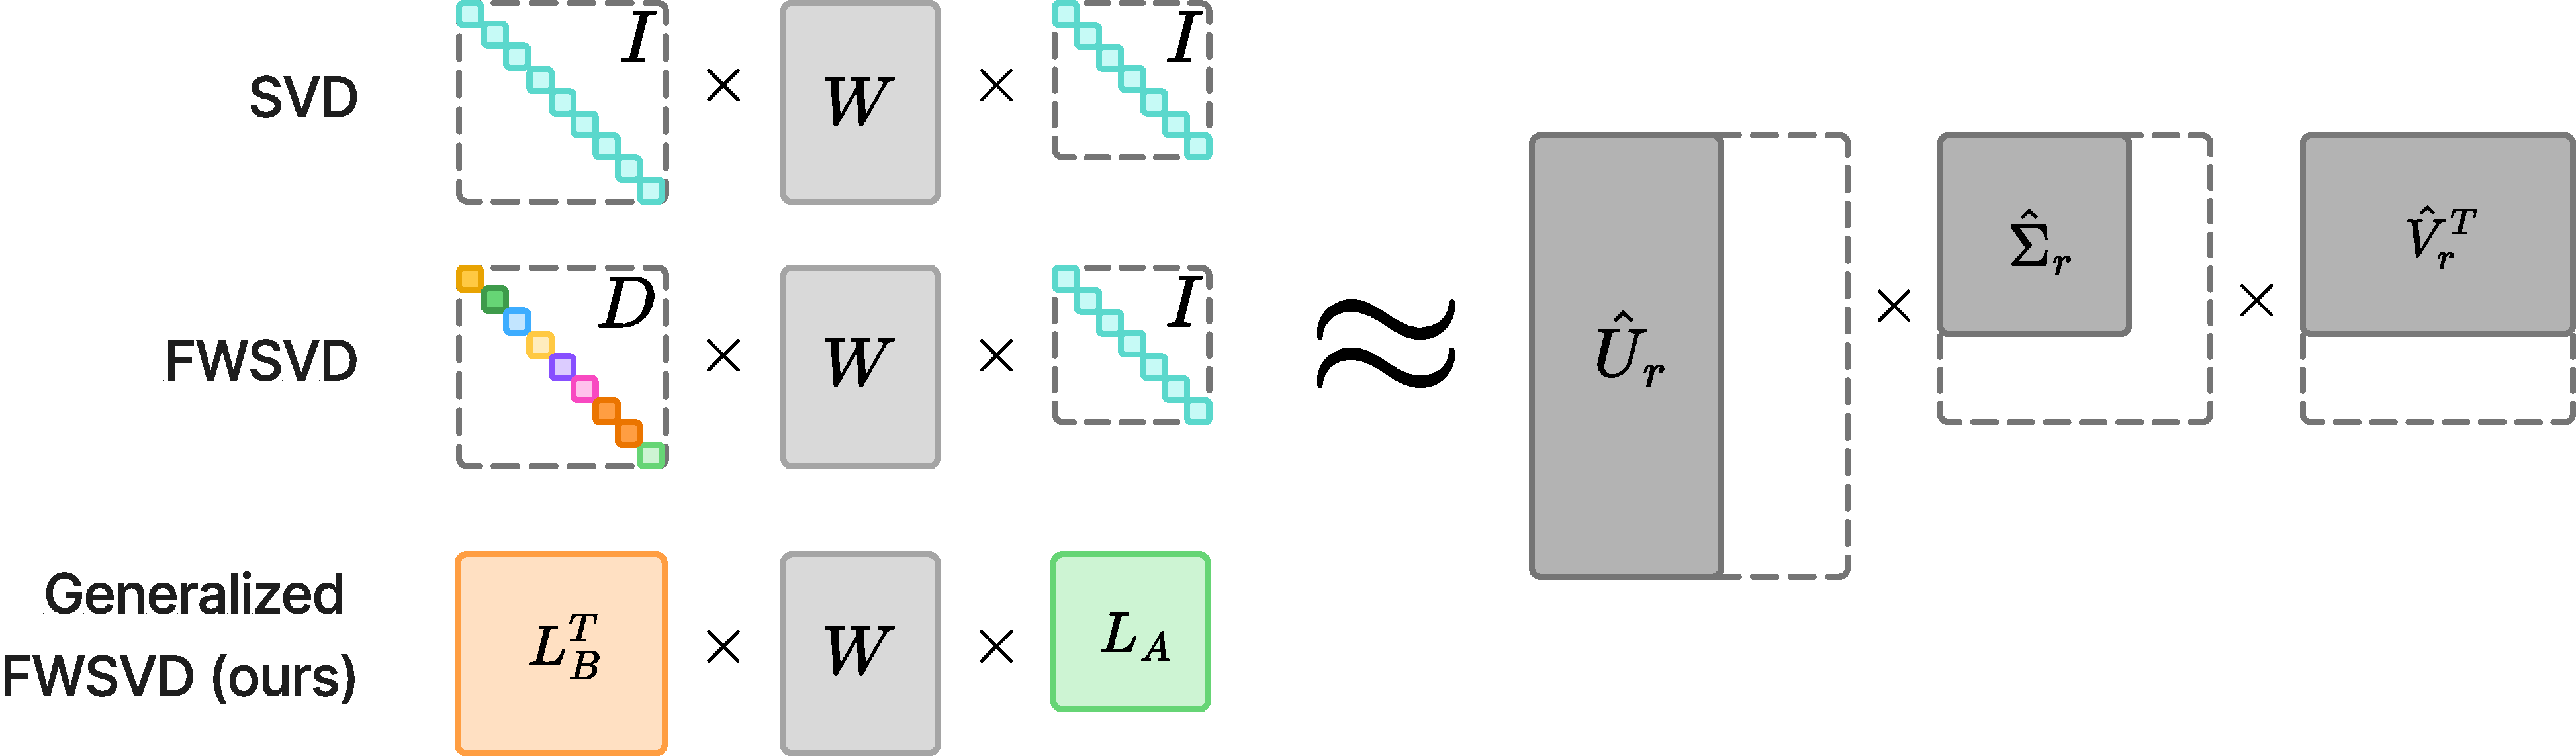
\includegraphics[clip, width=\linewidth]{figs/genfwsvd.pdf}
\caption{Generalization of the Weighted SVD frameworks.
For standard SVD, the transformation matrices are identity matrices. For FWSVD, the left matrix is diagonal but not identity, and the right matrix is identity. For GFWSVD, both matrices are non-diagonal.}
\label{fig:connection2fwsvd}
\end{figure}

\subsection{Relationship to Prior Works}
We show that FWSVD, presented in~\cite{FWSVD}, is a special case of our generalized framework.
The full justification is given in Appendix~\ref{sec:appendix0}. In FWSVD, the objective minimizes a weighted reconstruction error using a diagonal matrix $\mathbf{D}$ derived from a row-wise sum of the Fisher Information. We show that this setup corresponds to a diagonal Kronecker-factored approximation of the FIM, where $\mathbf{D}$ arises naturally from minimizing the Kronecker approximation error. The resulting solution for the low-rank factors $\mathbf{W}_2, \mathbf{W}_1$ matches that of FWSVD (up to a constant), which shows that their method is a special case of our more general framework. 

The connection between our generalized approach, the classical SVD and FWSVD is depicted in Figure~\ref{fig:connection2fwsvd}. Weighted SVD approaches can be interpreted as transforming the decomposed object—here, the weight matrix—into a new space where the low-rank approximation better aligns with the target task. In this formulation, the sensitivity matrices serve as transformation matrices that reweight the importance of different directions. Under this view, vanilla SVD corresponds to using identity transformations; FWSVD applies a diagonal (but non-identity) transformation on one side while keeping the other side as identity. In contrast, our method employs full, non-diagonal transformations on both sides, capturing richer structure in the parameter space.


\section{Kronecker Factorization Algorithm via Rank-1 SVD}
\label{sec:kron_algo}
%btaining a Kronecker approximation of $\mathbf{J}$ for an LLM layer using SVD-based standard algorithms~\cite{Loan1992} is very resource intensive due to the size of $\mathbf{J}$. In the Neural Network application, observed Fisher information is typically approximated using its expectation on data set samples and under the assumption that the rows and columns of the object $\mathbf{X}$ are independent~\cite{}. Such approximations


Suppose that we have a linear layer of a network with a weight matrix $\mathbf{W}$ and define $\mathbf{G}_i\in \mathbb{R}^{n \times m}$ as a weight gradients $\mathcal{L}(\theta)|_{\theta= \mathbf{W}}$  on the $i$-th batch, and $g_i = \vect({\mathbf{G}_i}) \in \mathbb{R}^{n \cdot m}$ - its flattening version.
Then, Fisher Information $\mathcal{I}_F(\theta)$ can be defined as an empirical mean over all batches in a dataset $D$:
\begin{equation}
 \mathcal{I}_F(\theta^{\star}) = \mathbb{E}\left[g g^\top\right] = \frac{1}{|D|}\sum_{i=1}^{|D|}{g}_{i}^{}{g}_{i}^\top.
 \label{eq:J}
\end{equation}

Kronecker product approximation is obtained by solving minimization problem:
\begin{equation}
\min \left\| \mathcal{I}_F - \mathbf{A} \otimes \mathbf{B} \right\|_{\operatorname{F}}
\label{eq:min_probles}
\end{equation}

Kronecker product decomposition of $\mathcal{I}_F$ is computed from a rank-1 approximation of permuted matrix $\tilde{\mathcal{I}}_F = \mathcal{R} \mathcal{I}_F \in \mathbb{R}^{m^2\times n^2}$, as it is described in~\cite{Loan1992}. The pseudocode of the method is in Algorithm~\ref{alg:kron-factors}. 

\begin{algorithm}[h]
\caption{Compute Kronecker Factors via Rank-1 SVD}
\label{alg:kron-factors}
\begin{algorithmic}[1]
\Require List of gradients $\{g_i\}_{i=1}^{|D|}$, $|D|$ -- number of batches
\State $\mathcal{I}_F \gets \frac{1}{|D|}\sum_{i=1}^{|D|}g_{i}g_{i}^T$
\State $\tilde{\mathcal{I}}_F \gets \mathcal{R} \mathcal{I}_F$ 
\State $(u, \sigma, v^\top) \gets$ Leading singular triplet \Comment{Truncated SVD}
\State $b \gets u \cdot \sigma$ \Comment{$b = \vect(\mathbf{B})$}
\State $a \gets v$ \Comment{$a = \vect(\mathbf{A})$}
\State $\mathbf{B} \gets \text{reshape}(b, (m, m))$
\State $\mathbf{A} \gets \text{reshape}(a, (n, n))$
\State \Return $(\mathbf{B}, \mathbf{A})$
\end{algorithmic}
\end{algorithm}

\subsection{Efficient Rank-1 Computation}
The primary computational bottleneck of Algorithm arises in performing SVD on the matrix $\mathcal{\tilde{I}}_F$.

Standard SVD is computationally intractable for large matrices, so we employ truncated SVD using the Lanczos~\cite{lanczos1950iteration} method, which avoids explicit matrix construction and requires only the ability to multiply the matrix with a vector from the left or right. Even in this setting, aggregating the full second-moment gradient information across all batch samples is computationally expensive. 

We can show (see  Appendix~\ref{sec:appendixa}) that permuted $\mathcal{I}_F$ for $i$-th batch can be defined as the Kronecker product of the corresponding gradient matrices:

\begin{equation}\label{eq:permuted_fisher}
\tilde{\mathcal{I}}_F = \frac{1}{|D|}\sum_{i=1}^{|D|} \mathbf{G}_i \otimes \mathbf{G}_i,
\end{equation}
then multiplication of this  matrix $\mathcal{\tilde{I}}_F$ to a vector $z$ from left will be:
\begin{equation}
\mathcal{\tilde{I}}_F z = \frac{1}{k}\left(\sum_{i=1}^{k} \mathbf{G}_i \otimes \mathbf{G}_i\right) z = \frac{1}{|D|}\left(\sum_{i=1}^{|D|} \mathbf{G}_i \otimes \mathbf{G}_i\right)\mathbf{Z} = z, \text{ where } z =  \vect(\mathbf{Z}), \mathbf{Z} \in \mathbb{R}^{n\times n} 
\end{equation}

Using property of the Kronecker product $(\mathbf{K}\otimes \mathbf{L}) \vect\left(\mathbf{C}) = \vect(\mathbf{K^\top} \mathbf{C} \mathbf{L}\right)$
%  \label{eq:kron_property}
% \end{equation}
we reduce the matrix-vector multiplication to a sequence of matrix multiplications. 
% involving matrices of size approximately $m\times n$:
\begin{equation}
\tilde{\mathcal{I}}_F z = \frac{1}{|D|}\sum_{i=1}^{|D|}  \vect(\mathbf{G}_i^\top \mathbf{Z} \mathbf{G}_i) 
\label{eq:matvec}
\end{equation}

% \begin{equation}
% \tilde{\mathcal{I}}_F^{\top} z = \frac{1}{|D|}\sum_{i=1}^{|D|} \vect(\mathbf{G_i} \mathbf{Z} \mathbf{G_i^\top}) 
% \label{eq:rmatvec}
% \end{equation}
The derivation for right-side multiplication is analogous (see Appendix~\ref{sec:appendixb}).
Using these operations, we can obtain an approximation of the Fisher information for layers of LLMs and batch sizes used in practice within a reasonable time.

\subsection{Time Complexity of the proposed Rank-1 Computation}

The time complexity of computing the truncated SVD of the matrix $\mathbf{\tilde{J}} \in \mathbb{R}^{m^2 \times n^2}$ consists of the cost of matrix-vector multiplications and the orthogonalization step. In the standard matrix-vector multiplication case, multiplying the Fisher matrix $\mathbf{\tilde{J}}$ by a vector has a cost of $\boldsymbol{\mathcal{O}}\left(m^2 n^2\right)$, while orthogonalization costs $\boldsymbol{\mathcal{O}}((m^2 + n^2) \cdot r^2)$, where $r$ is the rank of the decomposition and can typically be neglected. 

However, using the structured formulation from Eq.~\ref{eq:matvec}, where left matrix-vector products are implemented via multiplications with matrices $\mathbf{G}_i^\top \in \mathbb{R}^{m \times n}$, $\mathbf{Z} \in \mathbb{R}^{n \times n}$, and $\mathbf{G}_i \in \mathbb{R}^{n \times m}$, the overall complexity is reduced to $\boldsymbol{\mathcal{O}}\left(m n^2 + m^2 n\right)$. Applying analogous reasoning to the right matrix-vector products (see Eq.~\ref{eq:rmatvec}) one can yield the same complexity.

\begin{wrapfigure}{r}{0.42\textwidth}
  \centering
  \vspace{-10pt} % Adjust vertical spacing as needed
  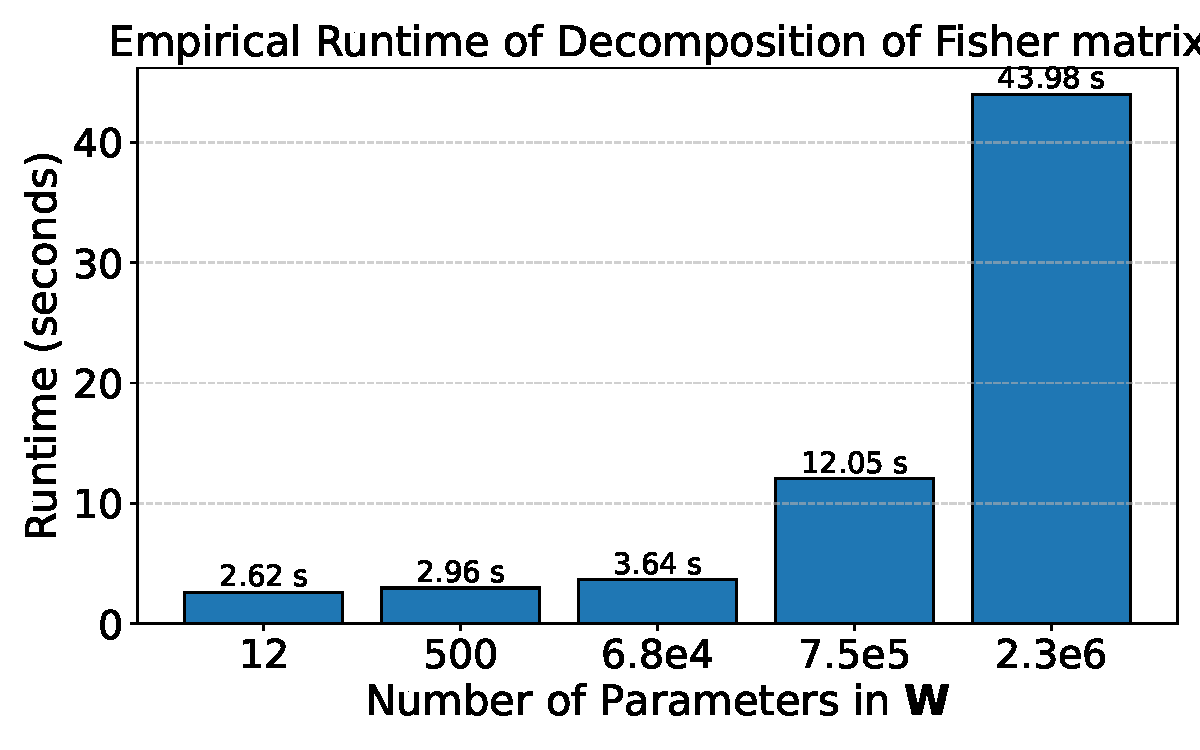
\includegraphics[width=0.40\textwidth]{figs/time_alg.pdf}
  \vspace{-10pt} % Adjust vertical spacing as needed
  \caption{Empirical runtime for computing the Kronecker decomposition of the Fisher matrix for weight matrices of varying sizes.}
  \label{fig:time_algo}
\end{wrapfigure}

Although the proposed method exhibits cubic complexity with respect to the dimensions of the linear layer’s weight matrix, its empirical runtime grows more slowly than that of the standard matrix-vector product, which scales quartically. In large language models, where $m$ and $n$ are typically on the order of $10^3$, this reduction yields a practically significant speedup. Table~\ref{fig:time_algo} reports the empirical decomposition times for $\mathcal{\tilde{I}}_F$, corresponding for matrices $\mathbf{W}$ with different sizes.


%\begin{table}[h]
%\centering
%\caption{empirical runtime of different approaches for computing $\mathbf{\tilde{J}}$ decomposition}
%\scalebox{0.8}{
%\begin{tabular}{lccccc}
%\toprule
%Method / Params & 12 & 500 & $6.8\cdot10^4$ & $7.5\cdot10^5$ & $2.3\cdot10^6$ \\
%\midrule
%Cuda JIT & 0.21 s & 0.42 s  & 18.08 s & 10.4 m & 2.34 h \\
%Ours (Algs.~\ref{alg:kron-factors}) & 2.62 s & 2.96 s & 3.64 s & 12.05 s & 43.98 s \\
%\bottomrule
%\end{tabular}}
%\label{tab:runtime_comparison}
%\end{table}





\section{Numerical Experiments}
\label{sec:experiments}

To validate our theoretical contributions, we conduct extensive numerical experiments on several transformer architectures: the encoder-only BERT model~\cite{bert} and the decoder-only LLM LLaMA 2~\cite{llama2}. Our goal is to demonstrate the practical benefits of GFWSVD in low-rank compression under fine-tuning and evaluation protocols. We conduct all experiments on a single NVIDIA A100 GPU with latest CUDA drivers using Python 3.12. The code is available on GitHub:~\href{https://github.com/sayankotor/FisherKronecker/tree/release}{link}.

%The code for the experiments, as well as the code for the Kronecker Factorization Algorithm, will be included in the supplementary material.
%The code is available on GitHub:~\href{https://github.com/sayankotor/FisherKronecker/tree/maxim}{link}.

% \begin{figure}[htbp!]
%     \centering
%     \vspace{-12pt} 
%     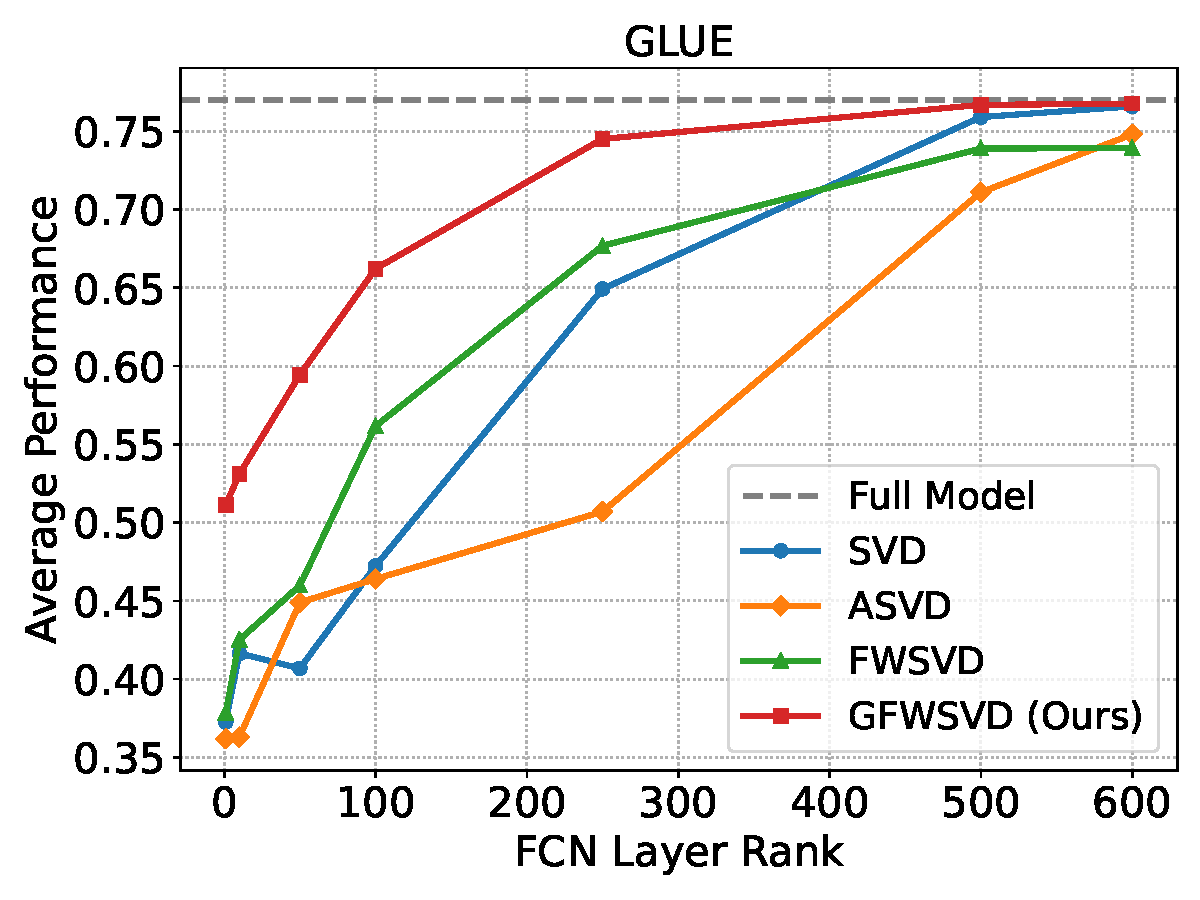
\includegraphics[width=.5\textwidth, trim=.3cm .3cm .3cm .3cm, clip]{figs/GLUE.pdf}
%     \caption{Macro-averaged GLUE performance of \texttt{bert-base-uncased} model for different compression ranks.}
%     \label{fig:bert_glue_avg}
%     \vspace{-12pt} 
% \end{figure}

% \begin{figure}[htbp!]
%     \centering
%     \vspace{-12pt} 
%     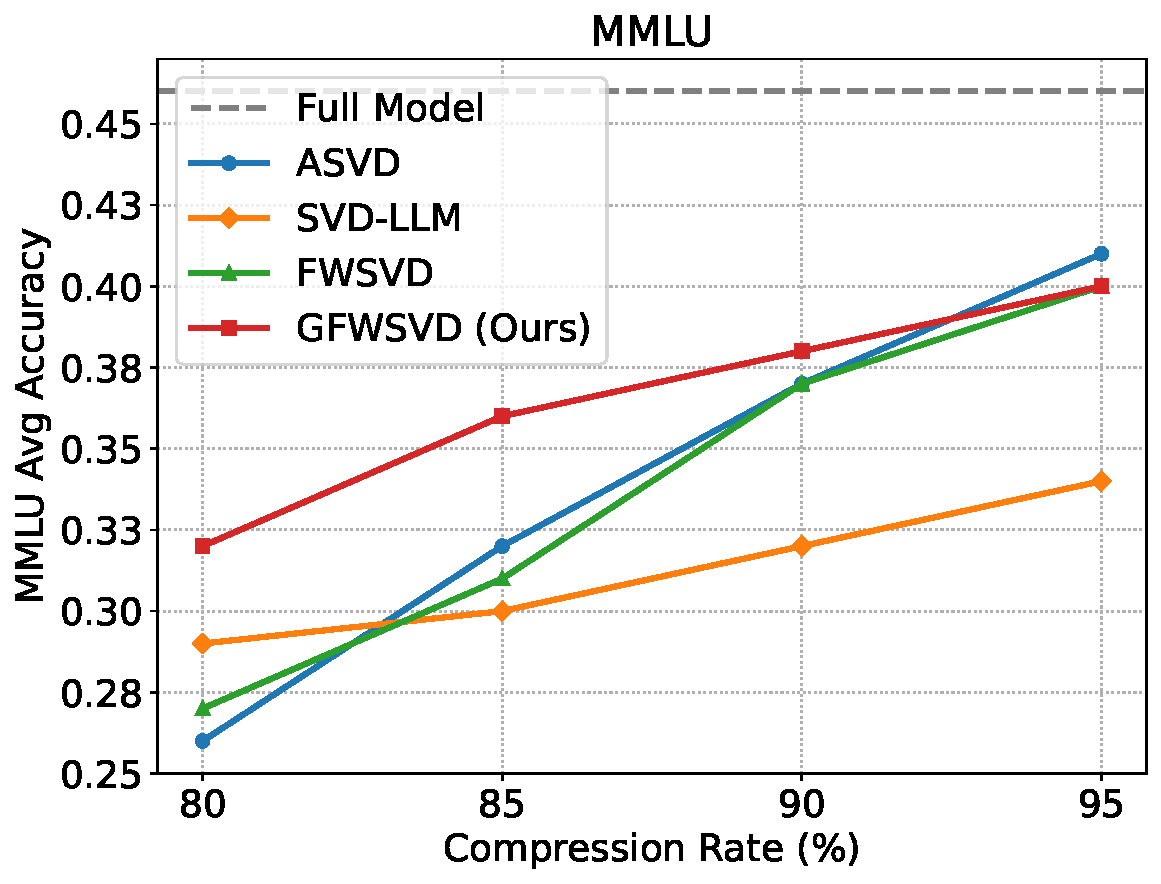
\includegraphics[width=.5\textwidth, trim=.3cm .3cm .3cm .3cm, clip]{figs/mmlu_avg_with_cr.pdf}
%     \caption{Macro-averaged GLUE performance of \texttt{bert-base-uncased} model for different compression ranks.}
%     \label{fig:mmlu_avg}
%     \vspace{-12pt} 
% \end{figure}

\begin{figure}[htbp!]
    \centering
    \vspace{-12pt}
    \begin{minipage}{0.49\textwidth}
        \centering
        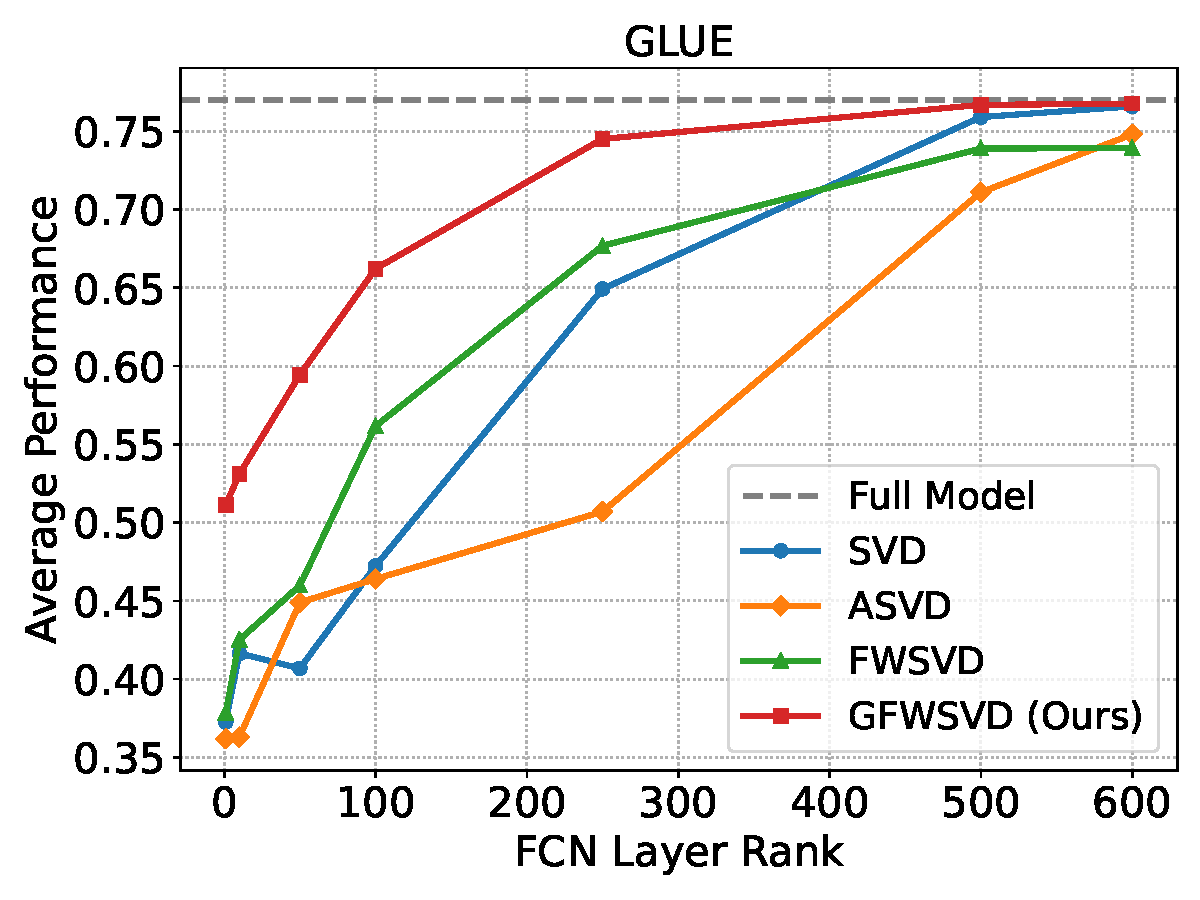
\includegraphics[width=\textwidth, keepaspectratio, trim=.3cm .3cm .3cm .3cm, clip]{figs/GLUE.pdf}
        \caption{Macro-averaged GLUE performance of \texttt{bert-base-uncased} model for different compression ranks.}
        \label{fig:bert_glue_avg}
    \end{minipage}
    \hfill
    \begin{minipage}{0.49\textwidth}
        \centering
        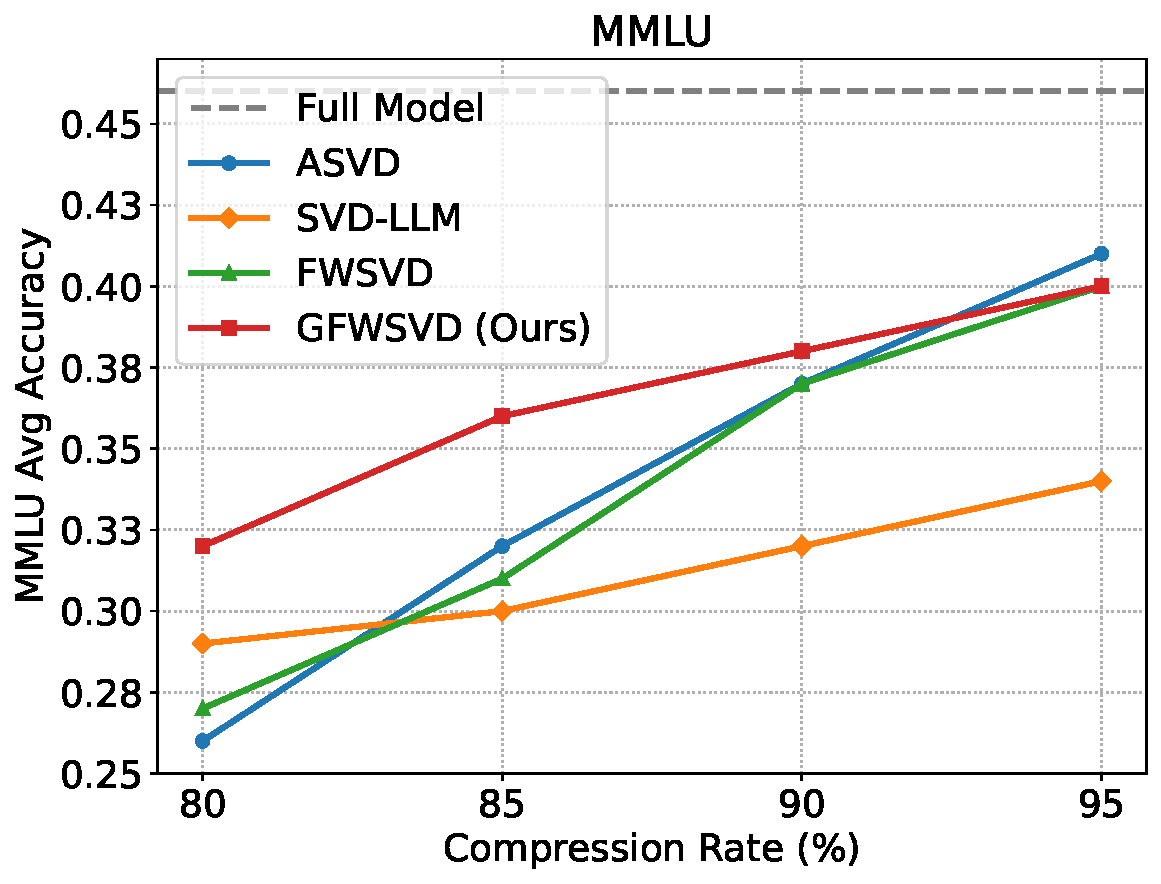
\includegraphics[width=\textwidth, keepaspectratio, trim=.3cm .3cm .2cm .3cm, clip]{figs/mmlu_avg_with_cr.pdf}
        \caption{Average MMLU performance of \texttt{llama-2-7b-chat} model for different compression rates.}
        \label{fig:mmlu_avg}
    \end{minipage}
    \vspace{-12pt}
\end{figure}


\subsection{Compressing the Transformer Encoder}
\label{sec:bert}


% We adopt a “fine-tune then compress” workflow akin to FWSVD~\cite{FWSVD}. Starting from the pre-trained \texttt{bert-base-uncased} checkpoint\footnote{\url{https://huggingface.co/google-bert/bert-base-uncased}}, we first fine-tune on each GLUE task~\cite{wang-etal-2018-glue}. Once task-specific weights are obtained, we apply low-rank factorization to all fully-connected layers—identified as the primary parameter bottleneck in BERT~\cite{chekalina-etal-2023-efficient}. For each task, we compress these linear blocks to a predetermined set of ranks (see Table~\ref{tab:bert_ranks}), enabling a systematic evaluation of accuracy versus model size.

% \begin{table}[htbp]
%   \centering
%   \caption{Macro-Averaged GLUE Performance Across Compression Levels}
%   \label{tab:glue_results}
%   \setlength{\tabcolsep}{1pt}
%   \begin{tabular}{lccccccc}
%     \toprule
%     Method / FCN Rank& 600 & 500 & 250 & 100 & 50 & 10 & 1 \\
%     \midrule
%     SVD            & 0.7659 & 0.7590 & 0.6493 & 0.4723 & 0.4069 & 0.4164 & 0.3726 \\
%     ASVD~\cite{asvd} & 0.7480 & 0.7110 & 0.5070 & 0.4640 & 0.4490 & 0.3630 & 0.3620 \\
%     FWSVD~\cite{FWSVD} & 0.7392 & 0.7389 & 0.6768 & 0.5616 & 0.4598 & 0.4251 & 0.3784 \\
%     GFWSVD (Ours)  & 0.7676 & 0.7668 & 0.7451 & 0.6622 & 0.5945 & 0.5310 & 0.5113 \\
%     \bottomrule
%   \end{tabular}
% \end{table}


In our experiments, we follow the “fine-tune then compress” pipeline, similar to FWSVD~\cite{FWSVD}. We begin by fine-tuning a pre-trained checkpoint\footnote{\url{https://huggingface.co/google-bert/bert-base-uncased}} of the BERT-base model on a specific downstream GLUE task. Optimal fine-tuning hyperparameters (e.g., learning rate, batch size) are selected for each task using the Optuna framework~\cite{akiba2019optuna}. During this stage, we also collect gradients to construct the FIM $\mathcal{I}_F$ and compute its Kronecker decomposition as described in Section~\ref{sec:kron_algo}.

Using the resulting Cholesky factors $\mathbf{L}_\mathbf{A}$ and $\mathbf{L}_\mathbf{B}$, we uniformly compress the fully connected layers of BERT by factorizing them into two smaller layers, following the method detailed in Section~\ref{sec:layer_comp_theory}. The chosen layer-wise ranks and the resulting overall compression rate of the model are summarized in Table~\ref{tab:bert_ranks}. We reproduce the ASVD method using the original authors’ code. For FWSVD, we incorporate the newly constructed FIM into the compression process.


\begin{table}[htbp!]
\label{rank_rate}
\centering
\caption{The correspondence between rank and entire BERT compression rate}
\label{tab:bert_ranks}
\begin{tabular}{ l | r  | l | r}
\toprule
Rank & C.Rate & Rank & C.Rate \\
\midrule
1 & $\sim 40\%$ & 100 & $\sim 33\%$\\
5 & $\sim 40\%$ & 250 & $\sim 23\%$ \\
10& $\sim 39\%$ & 500 & $\sim 8\%$\\
50& $\sim 36\%$ & 600 & $\sim 1\%$\\
\bottomrule
\end{tabular}
\end{table}



\begin{table}[htbp!]
  \vspace{-12pt}
  \centering
  \footnotesize
  \caption{Macro-averaged GLUE performance of the \texttt{bert-base-uncased} for different compression ranks. Best results for each rank are in \textbf{bold}.}
  \label{tab:glue_results}
  \setlength{\tabcolsep}{2pt}
  \begin{tabular}{lccccccc}
    \toprule
    Method / Rank & 600 & 500 & 250 & 100 & 50 & 10 & 1 \\
    \midrule
    SVD             & \textbf{0.77} & 0.76 & 0.65 & 0.47 & 0.41 & 0.42 & 0.37 \\
    ASVD~\cite{asvd}   & 0.75 & 0.71 & 0.51 & 0.46 & 0.45 & 0.36 & 0.36 \\
    FWSVD~\cite{FWSVD} & 0.74 & 0.74 & 0.68 & 0.56 & 0.46 & 0.43 & 0.38 \\
    GFWSVD (Ours)   & \textbf{0.77} & \textbf{0.77} & \textbf{0.75} & \textbf{0.66} & \textbf{0.59} & \textbf{0.53} & \textbf{0.51} \\
    \bottomrule
  \end{tabular}
  \vspace{-12pt}
\end{table}

We show average compression results in Table~\ref{tab:glue_results} and Figure~\ref{fig:bert_glue_avg}, extended results are in Appendix~\ref{appendix:glue} in Table~\ref{tab:glue_extended}. On most of the GLUE tasks and considered compression ranks, our proposed GFWSVD approach consistently outperforms both FWSVD and SVD, with particularly strong gains at lower ranks. While ASVD exhibits relatively poor performance on several tasks (QQP, QNLI), it occasionally surpasses GFWSVD — notably on SST2 under aggressive compression.

\subsection{Compressing the Transformer Decoder}
\label{sec:llamas}

We evaluate our approach on the decoder-only LLama 2 7B model\footnote{\url{https://huggingface.co/unsloth/llama-2-7b-chat}} against several competitive baselines: diagonal FI-based low-rank approximation method FWSVD~\cite{FWSVD}, and two activation-based methods -- ASVD~\cite{asvd} and SVD-LLM\cite{svdllm}. Notably, ASVD and SVD-LLM both rely on activation-based weighting to gauge parameter importance, while FWSVD and ours GFWSVD derive importance scores solely from gradient information. 

%Furthermore, SVD-LLM employs advanced heuristics for layer-wise budget allocation. In contrast, we stick to the idea of per-layer compression, leaving adaptive budget scheduling for future exploration.

We measure perplexity on WikiText 2~\cite{wikitext2} and PTB~\cite{ptb} datasets, and 5-shot reasoning performance on the MMLU benchmark~\cite{mmlu}. Following prior works on low-rank approximation of LLMs~\cite{svdllm, asvd}, we test several compression setups, removing from 5\% to 20\% of original parameters. 


Following standard practice in post-training LLM compression methods~\cite{svdllm, asvd}, we use a randomly sampled set of sentences as calibration data to generate gradients for further obtaining the factor matrices. For calibration data, we choose the FineWeb dataset~\cite{DBLP:conf/nips/PenedoKALMRW024} due to its high quality and diversity, and collect gradients on a random subsample of size 1024. These gradients are then used to obtain $\mathbf{L}_\mathbf{A}$ and $\mathbf{L}_\mathbf{B}$, as well as the data needed for FWSVD. As in LLMs, uniform layer compression can disproportionately degrade performance by over-compressing critical layers and under-utilizing redundancy in less sensitive ones, so it is essential for each method to use a compression configuration that accounts for layer sensitivity. For both ASVD and SVD-LLM, we used the corresponding code released by the authors and re-ran the necessary compression pipelines for our checkpoint with all hyperparameters set to default values. For our approach, we adopted the method of per-layer importance scores as described in the ASVD work.


%For FWSVD we uniformly compress all MLP layers of the model, while for our GFWSVD we adopted the appoach of per-layer importance scores as described in ASVD work. For both ASVD and SVD-LLM we used the corresponding code released by the authors and re-run the needed compression pipelines for our checkpoint with all the hyperparameters set to default values. 


% \todo[inline]{describe the experiments more carefully selection etc}

\begin{table*}[h]
\centering
\caption{Performance of the \texttt{unsloth/llama-2-7b-chat} compressed by various methods under compression ratios from 5\% to 20\% on WikiText-2, PTB, and MMLU. Lower is better for perplexity (\textcolor{green}{$\downarrow$}), higher is better for accuracy (\textcolor{green}{$\uparrow$}).}
\setlength{\tabcolsep}{1pt}
\resizebox{1\textwidth}{!}{%
\begin{tabular}{l|cc | c|ccccc}
\toprule
\textsc{Method} & WikiText-2\textcolor{green}{$\downarrow$} & PTB\textcolor{green}{$\downarrow$} & Compr. & MMLU Avg\textcolor{green}{$\uparrow$} & Humanities\textcolor{green}{$\uparrow$} & Other\textcolor{green}{$\uparrow$} & Social Sciences\textcolor{green}{$\uparrow$} & STEM\textcolor{green}{$\uparrow$} \\
\midrule
Full model & \textbf{6.94} & \textbf{25.75} & $100\%$ & 0.46 \scalebox{0.8}{$\pm$ 0.003} & 0.43 \scalebox{0.8}{$\pm$ 0.01} & 0.55 \scalebox{0.8}{$\pm$ 0.01} & 0.53 \scalebox{0.8}{$\pm$ 0.01} & 0.36 \scalebox{0.8}{$\pm$ 0.01} \\
\midrule
FWSVD~\cite{FWSVD} & 7.52 & 45.25 & \multirow{4}{*}{$95\%$} & 0.40 \scalebox{0.8}{$\pm$ 0.003} & 0.36 \scalebox{0.8}{$\pm$ 0.01} & 0.45 \scalebox{0.8}{$\pm$ 0.01} & 0.45 \scalebox{0.8}{$\pm$ 0.01} & 0.35 \scalebox{0.8}{$\pm$ 0.01} \\
% ASVD                 & 5.64 & 29.529 & & \textbf{0.44} $\pm$ 0.10 & 0.42 $\pm$ 0.10 & 0.51 $\pm$ 0.08 & 0.50 $\pm$ 0.08 & 0.36 $\pm$ 0.08 \\
ASVD~\cite{asvd} & 7.60 & \textbf{26.29} & & \textbf{0.41} \scalebox{0.8}{$\pm$ 0.004} & 0.37 \scalebox{0.8}{$\pm$ 0.01} & \textbf{0.48} \scalebox{0.8}{$\pm$ 0.01} & \textbf{0.46} \scalebox{0.8}{$\pm$ 0.01} & \textbf{0.35} \scalebox{0.8}{$\pm$ 0.01} \\
SVD-LLM~\cite{svdllm}& 8.80 & 51.28 & & 0.34 \scalebox{0.8}{$\pm$ 0.004} & 0.31 \scalebox{0.8}{$\pm$ 0.01} & 0.38 \scalebox{0.8}{$\pm$ 0.01} & 0.35 \scalebox{0.8}{$\pm$ 0.01} & 0.31 \scalebox{0.8}{$\pm$ 0.01} \\
GFWSVD~(Ours) & \textbf{7.16} & 28.55 & & 0.40 \scalebox{0.8}{$\pm$ 0.003} & \textbf{0.38} \scalebox{0.8}{$\pm$ 0.01} & 0.47 \scalebox{0.8}{$\pm$ 0.01} & 0.44 \scalebox{0.8}{$\pm$ 0.01} & 0.33 \scalebox{0.8}{$\pm$ 0.01} \\
\midrule
FWSVD~\cite{FWSVD} & 11.53 & 96.62 & \multirow{4}{*}{$90\%$} & 0.37 \scalebox{0.8}{$\pm$ 0.004} & 0.34 \scalebox{0.8}{$\pm$ 0.01} & 0.43 \scalebox{0.8}{$\pm$ 0.01} & 0.42 \scalebox{0.8}{$\pm$ 0.01} & 0.33 \scalebox{0.8}{$\pm$ 0.01} \\
% ASVD                 & -& - & & \textbf{0.41} $\pm$ 0.09 & 0.38 $\pm$ 0.09 & 0.48 $\pm$ 0.07 & 0.47 $\pm$ 0.07 & 0.35 $\pm$ 0.08 \\
ASVD~\cite{asvd} & 8.97 & 40.12 & & 0.37 \scalebox{0.8}{$\pm$ 0.004} & 0.33 \scalebox{0.8}{$\pm$ 0.01} & 0.42 \scalebox{0.8}{$\pm$ 0.01} & 0.40 \scalebox{0.8}{$\pm$ 0.01} & 0.33 \scalebox{0.8}{$\pm$ 0.01} \\
SVD-LLM~\cite{svdllm} & 9.69 & 60.82 & & 0.32 \scalebox{0.8}{$\pm$ 0.004} & 0.30 \scalebox{0.8}{$\pm$ 0.01} & 0.35 \scalebox{0.8}{$\pm$ 0.01} & 0.32 \scalebox{0.8}{$\pm$ 0.01} & 0.30 \scalebox{0.8}{$\pm$ 0.01} \\
GFWSVD~(Ours) & \textbf{8.77} & \textbf{36.44} & & \textbf{0.38} \scalebox{0.8}{$\pm$ 0.002} & \textbf{0.35} \scalebox{0.8}{$\pm$ 0.01} & \textbf{0.44} \scalebox{0.8}{$\pm$ 0.01} &\textbf{0.42} \scalebox{0.8}{$\pm$ 0.01} & \textbf{0.33} \scalebox{0.8}{$\pm$ 0.01} \\
\midrule
FWSVD~\cite{FWSVD} & 22.06 & 411.50 & \multirow{4}{*}{$85\%$} & 0.31 \scalebox{0.8}{$\pm$ 0.009} & 0.29 \scalebox{0.8}{$\pm$ 0.01} & 0.34 \scalebox{0.8}{$\pm$ 0.01} & 0.33 \scalebox{0.8}{$\pm$ 0.01} & 0.30 \scalebox{0.8}{$\pm$ 0.01} \\
% ASVD                 & 6.74 & 59.84 & & 0.35 $\pm$ 0.06 & 0.31 $\pm$ 0.06 & 0.40 $\pm$ 0.05 & 0.39 $\pm$ 0.06 & 0.33 $\pm$ 0.07 \\
ASVD~\cite{asvd} & 10.91 & 83.49 & & 0.32 \scalebox{0.8}{$\pm$ 0.003} & 0.30 \scalebox{0.8}{$\pm$ 0.01} & 0.33 \scalebox{0.8}{$\pm$ 0.01} & 0.32 \scalebox{0.8}{$\pm$ 0.01} & 0.30 \scalebox{0.8}{$\pm$ 0.01} \\
SVD-LLM~\cite{svdllm} & 10.36 & 72.58 & & 0.30 \scalebox{0.8}{$\pm$ 0.004} & 0.29 \scalebox{0.8}{$\pm$ 0.01} & 0.34 \scalebox{0.8}{$\pm$ 0.01} & 0.31 \scalebox{0.8}{$\pm$ 0.01} & 0.30 \scalebox{0.8}{$\pm$ 0.01} \\
GFWSVD~(Ours)& \textbf{10.06} & \textbf{42.19} & & \textbf{0.36} \scalebox{0.8}{$\pm$ 0.004} & \textbf{0.33} \scalebox{0.8}{$\pm$ 0.01} & \textbf{0.41} \scalebox{0.8}{$\pm$ 0.01} & \textbf{0.38} \scalebox{0.8}{$\pm$ 0.01} & \textbf{0.32} \scalebox{0.8}{$\pm$ 0.01} \\
\midrule
FWSVD~\cite{FWSVD} & 66.37 & 1523.00 & \multirow{4}{*}{$80\%$} & 0.27 \scalebox{0.8}{$\pm$ 0.004} & 0.25 \scalebox{0.8}{$\pm$ 0.01} &	0.30 \scalebox{0.8}{$\pm$ 0.01} & 0.28 \scalebox{0.8}{$\pm$ 0.01} & 0.28 \scalebox{0.8}{$\pm$ 0.01} \\
% ASVD                 & 8.91 & 114.70 & & 0.29 $\pm$ 0.00 & 0.27 $\pm$ 0.01 & 0.32 $\pm$ 0.01 & 0.30 $\pm$ 0.01 & 0.27 $\pm$ 0.01 \\
ASVD~\cite{asvd} & 27.73 & 241.57 & & 0.26 \scalebox{0.8}{$\pm$ 0.004} & 0.25 \scalebox{0.8}{$\pm$ 0.01} & 0.27 \scalebox{0.8}{$\pm$ 0.01} & 0.24 \scalebox{0.8}{$\pm$ 0.01} & 0.28 \scalebox{0.8}{$\pm$ 0.01} \\
SVD-LLM~\cite{svdllm} & 11.23 & 98.91 & & 0.29 \scalebox{0.8}{$\pm$ 0.004} & 0.27 \scalebox{0.8}{$\pm$ 0.01} & 0.32 \scalebox{0.8}{$\pm$ 0.01} & 0.29 \scalebox{0.8}{$\pm$ 0.01} & 0.29 \scalebox{0.8}{$\pm$ 0.01} \\
GFWSVD~(Ours)& \textbf{11.13} & \textbf{50.50} & & \textbf{0.32} \scalebox{0.8}{$\pm$ 0.003} & \textbf{0.30} \scalebox{0.8}{$\pm$ 0.01} & \textbf{0.35} \scalebox{0.8}{$\pm$ 0.01} & \textbf{0.34} \scalebox{0.8}{$\pm$ 0.01} & \textbf{0.30} \scalebox{0.8}{$\pm$ 0.01} \\
\bottomrule
\end{tabular}
}
\label{tab:llama2_compression}
\end{table*}
\hspace{-7pt}

Table~\ref{tab:llama2_compression} and Figure~\ref{fig:mmlu_avg} shows that GFWSVD consistently outperforms both simple and strong baselines across all compression rates. In particular, at the most aggressive settings (15–20\% of the original parameters), our method matches or exceeds the accuracy of activation-based methods and shows substantially lower perplexities on both WikiText-2 and PTB.

%Unlike ASVD and SVD-LLM, which in their final configurations apply light and uniform compression across all layers, our proposed GFWSVD method enables more targeted and aggressive compression in the layers where it has the greatest impact.

\section{Limitations}
\label{sec:limitations}
Our method decomposes the observed Fisher information matrix $\mathcal{I}_F$ into a Kronecker product of two smaller matrices, $\mathbf{Y}$ and $\mathbf{X}$ (Eq.~\ref{eq:min_probles}). While effective, this assumes exact factorization, which may not hold in practice and can limit approximation quality and task sensitivity. In LLM experiments, we also observed cases where the estimated Kronecker factors were singular, requiring regularization (e.g., $\mathbf{Y} \leftarrow \mathbf{Y} + \alpha \operatorname{diag}{\mathbf{Y}}$) to ensure positive definiteness and numerical stability. Although this resolves instability, it introduces additional computational overhead.

We observed that compression effectiveness varies significantly across layers, making preliminary layer selection necessary to achieve favorable trade-offs. A key limitation of our current approach is the lack of coordination across layers during compression. For effective multi -- layer compression—especially in large-scale models like LLMs -- it is important to account for cross-layer dependencies. Future work could focus on modeling these interactions to enable joint compression strategies.

\section{Broader impacts}
\label{sec:border_impact}

Our method, GFWSVD, enables more efficient compression of large language models, which can significantly reduce computational costs and energy consumption. This may help democratize access to powerful NLP tools and promote more sustainable AI deployment. However, as with any compression method, there is a risk of preserving harmful biases or weakening safety mechanisms. We advocate for responsible evaluation and deployment of compressed models, especially in sensitive applications.


\section{Conclusion and Future Work}

In this work we propose \textbf{Generalized Fisher-Weighted SVD (GFWSVD)}, a gradient-based low-rank approximation method that accurately incorporates parameter importance via the full FIM. Unlike the diagonal approximation of the FIM~\cite{FWSVD}, GFWSVD considers parameter correlations by leveraging a scalable Kronecker decomposition algorithm, and provides an optimal trade-off between downstream accuracy and computational efficiency. We thoroughly evaluate GFWSVD with encoder-only model BERT on GLUE benchmark and decoder only LLM LLaMa 2 on MMLU reasoning benchmark. We demonstrate GFWSVD’s superiority over diagonal Fisher- and activation-based SVD methods, particularly at extremely low ranks.

GFWSVD highlights the critical role of accurate FIM computation in compression. While our approach performs well empirically, its reliance on a rank-1 Kronecker approximation of the Fisher matrix may oversimplify important structure. Future work could explore higher-rank Kronecker series to capture richer task-relevant information, and extend the method to model cross-layer dependencies, potentially improving performance by leveraging transitive correlations across the network.

% ------------------------- PREVIOUS VERSION -------------------------
% In this work we present \textbf{Generalized Fisher-Weighted SVD (GFWSVD)}, a novel gradient-based method of a weighted low-rank approximation. GFWSVD accurately captures parameter importance by using the full observed FIM. Unlike FWSVD, a prior method that relies on diagonal approximations and ignore parameter correlations, GFWSVD incorporates both diagonal and off-diagonal elements using a Kronecker approximation. To mitigate computational challenges, we introduce a scalable variant of the Kronecker decomposition algorithm, reducing complexity while preserving the expressiveness of the full Fisher structure.

% Our compression approach preserves fine-grained task sensitivity and achieves superior accuracy retention compared to existing weighted SVD methods -- both those guided by Fisher information and those based on activation statistics. We evaluate GFWSVD on both encoder- and decoder-based Transformer models: BERT on the GLUE benchmark and LLaMa2-7B-chat on MMLU. Empirical results show that GFWSVD consistently outperforms existing low-rank compression baselines across standard tasks. %In decoder-based models, our method delivers particularly strong gains at low-rank compression levels. On MMLU, GFWSVD improves both perplexity and output quality, trailing only ASVD at the 5% compression level. At 20% compression, GFWSVD outperforms Fisher-Weighted SVD by 5%, SVD-LLM by 3%, and ASVD by 6%.

% These results validate the importance of modeling parameter correlations in Fisher-based compression methods and highlight the potential of GFWSVD as an efficient and effective tool for post-training model compression. Future work may explore extending this framework to structured pruning or joint quantization-compression pipelines.

% While our approach demonstrates strong empirical performance, it relies on a rank-1 Kronecker product approximation of the Fisher information matrix, which may oversimplify the underlying structure and lead to information loss. Hence, a promising direction for future research is to explore and efficiently incorporate Kronecker product-based approximation series of higher rank, capturing more nuanced task-related information. Additionally, generalizing the method to capture cross-layer dependencies, rather than focusing solely on individual layers, could further improve performance by modeling valuable transitive correlations that better reflect the structural properties of the network.
% ------------------------- PREVIOUS VERSION -------------------------


%Our compression approach based on the Kronecker product approximation of the Fisher Information matrix retains finer-grained task sensitivity and achieves higher accuracy retention compared to existing SVD and Fisher-Weighted SVD  methods. 

%The overall richer formulation is designed to better capture parameter correlations across rows and columns of the weight matrix and guide a more optimal dimensionality reduction. This extended weighting strategy ensures that compression does not merely prioritize individual parameters in isolation but instead accounts for global structural dependencies within the weight matrix. The resulting factorization retains more relevant task information, improving model accuracy under higher compression rates while maintaining computational efficiency.

% we propose a more accurate weighted SVD method, called Generalized Fisher-Weighted SVD (GFWSVD), which better aligns with the model’s learned representations.




\newpage

%\section{Fisher Matrices of low-rank matrices in the LoRA approach}
%$$\Delta W = BA$$
%$LT$, $R$ - left and right factors
%$$LT @ \Delta W @ R = LT @ B@  A@ R $$
%$$LT @ B = ( QR \text{ decomp} )= Q_B R_B $$
%$$R.T @ A.T = ( QR \text{ decomp} )= Q_A R_A $$
%$$ R_B @ R_A.T  = U \Sigma V_t $$
%$$\hat U = Q_B U$$
%$$\hat V_t =  V_t Q_A.T$$
%new updates:
%$$\Delta W_{new} =\hat{U} \Sigma \hat{V_t}  $$

\bibliographystyle{plainnat}
\bibliography{neurips_2024}

\appendix
\section{Appendix A: Special case of diagonal Fisher Information Matrix}
\label{sec:appendix0}
In this section, we show that FWSVD, presented in~\cite{FWSVD}, is a special case of our generalized approach. 

In the work of~\cite{FWSVD}, authors propose to minimize the following objective:
\begin{equation}\label{eq:fwsvd}
    \underset{\mathbf{W_1,W_2}}{\min}  \left\| 
    \mathbf{D}\mathbf{W}^{\star} - \mathbf{D}\mathbf{W_2}\mathbf{W_1} \right\| _F^2
\end{equation} where $\mathbf{D}$ is the diagonal matrix $\sqrt {\operatorname{diag}\left(\mathbb{E} [\mathbf{G} \mathbf{G}^\top] \right)}$.
Specifically, $\mathbf{D}_{i,i} = \sqrt{\sum_{j=1}^m \mathbb{E} (\mathbf{G}_{i,j})^2 }$.
% The solution takes the following form: $\mathbf{W}_2 = \mathbf{D}^{-1} \mathbf{U}_r \sqrt{\mathbf{S}_r}$,   $\mathbf{W}_1 = \sqrt{\mathbf{S}_r} \mathbf{V}^\top_r $.

% Lets consider $\mathbf{D}^2 = \mathbf{D}\mathbf{D}^T$ of size $n \times n$ and define $e = \left[ 1, \dots, 1 \right]$ - a vector of ones of length $m$. Then, the diagonal of $\mathbf{D}^2$ can be written as $\mathbf{D}e$. 

Similarly to~\ref{eq:min_probles}, we approximate the Fisher Information with a Kronecker product of identity matrix $\mathbf{I}_m$ and some diagonal matrix $\mathbf{\tilde{D}}$.
As described further in Section~\ref{sec:kron_algo} and Appendix~\ref{sec:appendixa}, under the permutation $\mathcal{R}$, the problem 
\begin{equation}\label{eq:diagonal_kronecker_approx}
    \underset{\mathbf{D}}{\min}  \left\| \mathbf{I}_F - \mathbf{I}_m \otimes \mathbf{\tilde{D}} \right\|_{\operatorname{F}}
\end{equation}
reduces to minimization of the expression
\begin{equation}\label{eq:diagonal_kronecker_approx_reshaped}
    \underset{\mathbf{d}}{\min} \left\| \mathbb{E} [\mathbf{G} \otimes \mathbf{G}]  - (\mathbf{I}_n \odot \mathbf{I}_n) d \cdot  \mathrm{vec} (\mathbf{I}_m)^\top \right\|_{\operatorname{F}}
\end{equation}
where $\odot$ is a Khatri-Rao product (column-wise Kronecher product) and $\cdot$ is a vector outer product; $d$ is a vector diagonal of $\mathbf{\tilde{D}}$; $\mathbb{E} [\mathbf{G} \otimes \mathbf{G}]$ is a permuted Fisher Information matrix  $\mathbf{\tilde{I}_F}$, defined in Eq~\ref{eq:permuted_fisher}. 

For simplicity, we will use a shorter notation. Let $ \mathbf{E} = \mathbb{E} [\mathbf{G} \otimes \mathbf{G}] $, $ \mathbf{Z} = \mathbf{I}_n \odot \mathbf{I}_n$, $v =  \mathrm{vec} (\mathbf{I}_m)$. Then, the problem~\ref{eq:diagonal_kronecker_approx_reshaped} is equivalent to
\begin{equation}
    \underset{\mathbf{d}}{\min} \left\|  \mathbf{Z} d \cdot v^\top  - \mathbf{E} \right\|_{\operatorname{F}}
\end{equation}
Applying first-order optimality conditions yields:
\begin{gather*}
    \langle \mathbf{Z} \delta d \cdot v^\top, \mathbf{Z} d \cdot v^\top  - \mathbf{E} \rangle = 0 \\
    \langle \delta d \cdot v^\top, \mathbf{Z}^\top \mathbf{Z} d \cdot v^\top  - \mathbf{Z}^\top\mathbf{E} \rangle = 0 \\
    \langle \delta d , \mathbf{Z}^\top \mathbf{Z} d \cdot v^\top v  - \mathbf{Z}^\top\mathbf{E}v \rangle = 0 \\
\end{gather*}

Since $\mathbf{Z}^\top \mathbf{Z} = \mathbf{I}_n$, $v^\top v = \left\| v \right\|^2_2 = \left\|  \mathrm{vec}(\mathbf{I}_m) \right\|^2_2 = m$ , we have:

\begin{equation}
    d = \frac{1}{m}  (\mathbf{I}_n \odot \mathbf{I}_n)^\top \mathbb{E} [\mathbf{G} \otimes \mathbf{G}] \mathrm{vec}(\mathbf{I}_m) = \frac{1}{m}  (\mathbf{I}_n \odot \mathbf{I}_n)^\top \mathrm{vec}(\mathbb{E} [G G^\top] ) = \frac{1}{m} \operatorname{diag} (\mathbb{E} [G G^\top] )
\end{equation}

Thus, diagonal matrix $\mathbf{\tilde{D}}$ from Kronecker product approximation problem~\ref{eq:diagonal_kronecker_approx} equals square of matrix $\mathbf{D}$ from the FWSVD formulation~\ref{eq:fwsvd} up to the constant $\frac{1}{m}$.
% Since constant multiplier does not affect the solution to minimization problem, we can multiply 

We apply Theorem~\ref{th:ABsolution} to find factors $\mathbf{W}_2$, $\mathbf{W}_1$ for the obtained approximation $\mathbf{I}_F = \mathbf{I}_m \otimes \mathbf{\tilde{D}}$:
\begin{equation}
    \mathbf{W}_2 = \sqrt{\mathbf{\tilde{D}}}^{-1} \mathbf{\hat{U}}_r \sqrt{\mathbf{\hat{S}}_r} = \mathbf{D}^{-1} \mathbf{\hat{U}}_r \sqrt{\mathbf{\hat{S}}_r},  \mathbf{W}_1 = \sqrt{\mathbf{\hat{S}}_r} \mathbf{\hat{V}}^\top_r
\end{equation}
where  $\mathbf{\hat{U}}_r \mathbf{\hat{S}}_r \mathbf{\hat{V}}^\top_r $ is r-rank SVD of $\mathbf{\sqrt{\tilde{D}}W}^\star = \mathbf{DW}^\star$.
This is the same solution that minimizes the problem~\ref{eq:fwsvd} from FWSVD paper~\cite{FWSVD}. Consequently, FWSVD approach is a special case of diagonal Kronecker product approximation of Fisher Information.

\section{Appendix B: Additional Explanations for Kronecker decomposition adaptation}
\label{sec:appendixa}
% Add your appendix content here
Let's show that the permuted \( \mathcal{I}_F \) in the Kronecker decomposition algorithm can be expressed as the Kronecker product of the corresponding gradient matrices.

We start with the empirical Fisher information matrix defined as:


\begin{equation}
\mathcal{I}_F = \frac{1}{|D|}\sum_{i=1}^{|D|}{g}_{i}^{}{g}_{i}^\top.
\end{equation}

and its reordered version:
 
\begin{equation}
\label{eq:reordered_IF}
   \tilde{\mathcal{I}}_F = \mathcal{R} \mathcal{I}_F
\end{equation}


% Using the identity
% \[
% \operatorname{vec}(\bm{g}_i \bm{g}_i^\top) = \bm{g}_i \otimes \bm{g}_i,
% \]
% we obtain:

% \begin{equation}
% \operatorname{vec}(\mathcal{I}_F)
% = \frac{1}{|D|} \sum_{i=1}^{|D|} \operatorname{vec}(\bm{g}_i \bm{g}_i^\top)
% = \frac{1}{|D|} \sum_{i=1}^{|D|} \bm{g}_i \otimes \bm{g}_i = \frac{1}{|D|} \sum_{i=1}^{|D|} \vect(\mathbf{G}_i) \otimes \vect(\mathbf{G}_i).
% \end{equation}

Using the identity
$$
\operatorname{vec}(\bm{g}_i \bm{g}_i^\top) = \bm{g}_i \otimes \bm{g}_i,
$$
we obtain:

\begin{equation}
\operatorname{vec}(\mathcal{I}_F) 
= \frac{1}{|D|} \sum_{i=1}^{|D|} \operatorname{vec}(\bm{g}_i \bm{g}_i^\top) 
= \frac{1}{|D|} \sum_{i=1}^{|D|} (\bm{g}_i \otimes \bm{g}_i).
\end{equation}

Let \( \mathcal{P} \in \mathbb{R}^{(ab)^2 \times (ab)^2} \) be the unique permutation matrix such that for any matrices \( \mathbf{A}, \mathbf{B} \in \mathbb{R}^{a \times b} \):

\begin{equation}
\mathcal{P} \cdot \operatorname{vec}(\mathbf{A} \otimes \mathbf{B}) = (\operatorname{vec}(\mathbf{A}) \otimes \operatorname{vec}(\mathbf{B})).
\end{equation}

Using this definition, we can write:

\begin{equation}
\mathcal{P} \cdot \operatorname{vec}(\mathbf{G}_i \otimes \mathbf{G}_i) = \operatorname{vec}(\mathbf{G}_i) \otimes \operatorname{vec}(\mathbf{G}_i).
\end{equation}

Therefore, the vectorized Fisher information becomes:

\begin{equation}
\operatorname{vec}(\mathcal{I}_F) = \frac{1}{|D|} \sum_{i=1}^{|D|} \mathcal{P} \cdot \operatorname{vec}(\mathbf{G}_i \otimes \mathbf{G}_i) = \mathcal{P} \cdot \operatorname{vec} \left( \frac{1}{|D|} \sum_{i=1}^{|D|}(\mathbf{G}_i \otimes \mathbf{G}_i) \right) = \mathcal{P}  \vect(\tilde{\mathcal{I}}_F) .
\end{equation}

So, $\tilde{\mathcal{I}}_F$ can be defined as $\frac{1}{|D|} \sum_{i=1}^{|D|}(\mathbf{G}_i \otimes \mathbf{G}_i)$. This fact is used in the accelerated adaptation of the Kronecker Factorization algorithm.

Now, suppose a $\mathcal{I}_F$ and $\tilde{\mathcal{I}}_F$ are connected with \( \mathcal{R} \in \mathbb{R}^{n \times n} \) (see Eq.~\ref{eq:reordered_IF}):


\begin{equation}
\operatorname{vec}(\widetilde{\mathcal{I}}_F) = (I \otimes \mathcal{R}) \cdot \operatorname{vec}(\mathcal{I}_F), \mathcal{P} = I \otimes \mathcal{R}
\end{equation}

%We can show~(see. Appendix A) that $\mathbf{\tilde{J}}$ in terms of weight gradients can be defined as:
%\begin{equation}
%    \mathbf{\tilde{I_F}} = \frac{1}{|D|}\sum_{i=0}^{|D|}(\vect^{-1}{g}_{i},\vect^{-1}{g}_{i}^T) = \frac{1}{|D|}\sum_{i=0}^{|D|}%(\mathbf{G_{i}},\mathbf{G_{i}}^T),
%    \label{eq:permuted_J}
%\end{equation}



%\begin{equation}
%    min \left\|\left| \mathbf{\tilde{J}} - \vect(\mathbf{Y})\vect(\mathbf{X})^T\right|\right|_{\operatorname{F}},
%\label{eq:min_to_approx_problem}
%\end{equation}

%Defining $P$ using the commutation matrix $\mathbf{K^{(m, n)}}$ $P = \mathbf{I_n} \otimes \mathbf{K^{(m, n)}} \otimes \mathbf{I_m}$ %we can rewrite Eq.~\ref{eq:min_probles} as
%$$
%\vect(\mathbf{Y}\otimes \mathbf{X}) = P(\vect(\mathbf{Y})\otimes \vect(\mathbf{X}))
%$$

%$$
% \vect^{-1} P^{-1} \vect(\mathbf{Y}\otimes \mathbf{X}) = \vect^{-1}(\vect(\mathbf{Y})\otimes \vect(\mathbf{X})) = \vect^{-1} (\vect y \otimes \vect x) =
%xy^\top= \mathbf{\tilde{J}}, $$


%\begin{equation}
%vec(\mathbf{J}) = P vec(\mathcal{\hat{J}})
%\end{equation}
%So,
%\begin{equation}
%\mathbf{\tilde{J}} =  xy^\top\approx \sum_{j=0}^{1} u_i \sigma_i v^T_i = x^{\star} \otimes \left(y^{\star}\right)^T
%\end{equation}

%To find Kronecker factors $\mathbf{Y}, \mathbf{X}$, we need to find $x^{\star} y^{T\star}$ using SVD decomposition of $\mathbf{\hat{J}}$ and reshape them: 
%\begin{equation}
%    \mathbf{Y} \approx \vect^{-1} (y^{\star}), \mathbf{X} \approx \vect^{-1} (x^{\star})
%    \label{eq:kron_factors}
%\end{equation}
%As defined is Eq.~\ref{eq:permuted_matrix_def}:
% \begin{equation}
% \mathbf{\hat{J}} = \mathcal{R} \frac{1}{|D|}\sum_{i=0}^{|D|}(\vec{g}_{i},\vec{g}_{i}^T) = \frac{1}{|D|}\sum_{i=0}^{|D|}\mathcal{R}(\vec{g}_{i}, \vec{g}_{i}^T)  = \frac{1}{|D|}\sum_{i=0}^{|D|}(vec^{-1} \vec{g}_{i}, vec^{-1} \vec{g}_{i}^T) = \frac{1}{|D|}\sum_{i=0}^{|D|}(\mathbf{{G}_{i}}\otimes\mathbf{{G}_{i}})
% \end{equation}

%\begin{align}
%\mathbf{\hat{J}} 
%= \mathcal{R} \cdot \frac{1}{|D|} \sum_{i=0}^{|D|} \left( \vec{g}_{i} \vec{g}_{i}^\top \right)
%= \frac{1}{|D|} \sum_{i=0}^{|D|} \mathcal{R} \left( \vec{g}_{i}, \vec{g}_{i}^\top \right)
%= \\
%=\frac{1}{|D|} \sum_{i=0}^{|D|} \left( \mathrm{vec}^{-1}(\vec{g}_{i}) \otimes \mathrm{vec}^{-1}(\vec{g}_{i}^\top) \right)
%= \frac{1}{|D|} \sum_{i=0}^{|D|} \left( \mathbf{G}_{i} \otimes \mathbf{G}_{i} \right)
%\end{align}


\section{Appendix C: Right vector-matrix multiplication}
\label{sec:appendixb}
We can define right vector-matrix multiplication as follows:
\begin{equation}
\mathcal{I}_F^\top z = (\sum_{i=1}^{|D|} \mathbf{G}_i \otimes \mathbf{G}_i)^\top z
\end{equation}

Using property of the Kronecker product $(\mathbf{K}\otimes \mathbf{L}) \vect(\mathbf{C}) = \vect(\mathbf{K^\top} \mathbf{C} \mathbf{L})$:
\begin{equation}
\label{eq:rmatvec}
\mathcal{I}_F^\top z = \sum_{i=1}^{|D|} \vect(\mathbf{G}_i \mathbf{Z} \mathbf{G}_i^\top) \text{, where } z =  \vect(\mathbf{Z}), \mathbf{Z} \in \mathbb{R}^{m\times m} 
\end{equation}

\section{Appendix D: Extended GLUE results}
\label{appendix:glue}

We report extended compression results on tasks of GLUE benchmark in Table~\ref{tab:glue_extended}.

\begin{table*}[htbp]
\centering
\caption{Performance of \texttt{bert-base-uncased} compressed by various methods under compression rates from 60\% to 99\% on GLUE benchmark. Lower is better for COLA (\textcolor{green}{$\downarrow$}), higher is better for all other tasks (\textcolor{green}{$\uparrow$}).}
% \setlength{\tabcolsep}{1pt}
\footnotesize
\begin{tabular}{l|ccccccccc}
\toprule
\textsc{Method / Dataset} & MRPC\textcolor{green}{$\uparrow$} & STSB\textcolor{green}{$\uparrow$} & QQP\textcolor{green}{$\uparrow$} & MNLI\textcolor{green}{$\uparrow$} & QNLI\textcolor{green}{$\uparrow$} & RTE\textcolor{green}{$\uparrow$} & COLA\textcolor{green}{$\downarrow$} & SST2\textcolor{green}{$\uparrow$} \\
\midrule
Full model & \textbf{0.77} & \textbf{0.87} & \textbf{0.90} & \textbf{0.83} & \textbf{0.90} & \textbf{0.56} & \textbf{0.41} & \textbf{0.91} \\
\midrule
& \multicolumn{8}{c}{Compression Rate $99\%$ ($r=600$)} \\
\midrule
SVD & 0.67 & 0.84 & 0.90 & 0.67 & 0.90 & 0.56 & 0.58 & 0.91 \\
ASVD~\cite{asvd} & 0.72 & 0.73 & 0.89 & 0.83 & 0.90 & 0.56 & 0.41 & 0.91 \\
FWSVD~\cite{FWSVD} & 0.72 & 0.87 & 0.90 & 0.72 & 0.90 & 0.55 & 0.36 & 0.91 \\
GFWSVD (Ours) & \textbf{0.73} & \textbf{0.87} & \textbf{0.90} & \textbf{0.73} & \textbf{0.90} & \textbf{0.56} & \textbf{0.55} & \textbf{0.92} \\
\midrule
& \multicolumn{8}{c}{Compression Rate $92\%$ ($r=500$)} \\
\midrule
SVD & 0.53 & 0.82 & 0.89 & 0.53 & 0.90 & 0.54 & 0.53 & 0.89 \\
ASVD~\cite{asvd} & 0.71 & 0.56 & 0.86 & 0.81 & 0.89 & 0.53 & 0.44 & 0.88 \\
FWSVD~\cite{FWSVD} & 0.71 & 0.87 & 0.90 & 0.71 & 0.89 & 0.56 & 0.34 & 0.91 \\
GFWSVD (Ours) & \textbf{0.73} & \textbf{0.87} & \textbf{0.90} & \textbf{0.73} & \textbf{0.90} & \textbf{0.56} & \textbf{0.49} & \textbf{0.92} \\
\midrule
& \multicolumn{8}{c}{Compression Rate $77\%$ ($r=250$)} \\
\midrule
SVD & 0.49 & 0.68 & 0.81 & 0.49 & 0.85 & 0.50 & 0.17 & 0.57 \\
ASVD~\cite{asvd} & 0.69 & 0.08 & 0.76 & 0.50 & 0.58 & 0.47 & 0.11 & 0.75 \\
FWSVD~\cite{FWSVD} & 0.69 & 0.86 & 0.89 & 0.69 & 0.89 & 0.61 & 0.23 & 0.80 \\
GFWSVD (Ours) & \textbf{0.71} & \textbf{0.86} & \textbf{0.89} & \textbf{0.71} & \textbf{0.89} & \textbf{0.61} & \textbf{0.38} & \textbf{0.88} \\
\midrule
& \multicolumn{8}{c}{Compression Rate $67\%$ ($r=100$)} \\
\midrule
SVD & 0.32 & 0.08 & 0.64 & 0.32 & 0.80 & 0.51 & 0.01 & 0.49 \\
ASVD~\cite{asvd} & 0.58 & 0.07 & 0.74 & 0.39 & 0.50 & 0.47 & 0.05 & 0.82 \\
FWSVD~\cite{FWSVD} & 0.69 & 0.58 & 0.87 & 0.71 & 0.86 & 0.55 & 0.21 & 0.72 \\
GFWSVD (Ours) & \textbf{0.71} & \textbf{0.70} & \textbf{0.87} & \textbf{0.71} & \textbf{0.86} & \textbf{0.55} & \textbf{0.21} & \textbf{0.72} \\
\midrule
& \multicolumn{8}{c}{Compression Rate $64\%$ ($r=50$)} \\
\midrule
SVD & 0.32 & 0.19 & 0.57 & 0.32 & 0.78 & 0.48 & 0.02 & 0.49 \\
ASVD~\cite{asvd} & 0.68 & -0.03 & 0.73 & 0.49 & 0.76 & 0.51 & -0.03 & 0.80 \\
FWSVD~\cite{FWSVD} & 0.69 & 0.65 & 0.84 & 0.69 & 0.72 & 0.46 & 0.03 & 0.77 \\
GFWSVD (Ours) & \textbf{0.69} & \textbf{0.65} & \textbf{0.84} & \textbf{0.69} & \textbf{0.72} & \textbf{0.46} & \textbf{0.05} & \textbf{0.77} \\
\midrule
& \multicolumn{8}{c}{Compression Rate $61\%$ ($r=10$)} \\
\midrule
SVD & 0.32 & 0.32 & 0.67 & 0.32 & 0.61 & 0.51 & 0.00 & 0.49 \\
ASVD~\cite{asvd} & 0.61 & -0.14 & 0.64 & 0.40 & 0.57 & 0.49 & -0.04 & 0.76 \\
FWSVD~\cite{FWSVD} & 0.37 & 0.32 & 0.79 & 0.37 & 0.57 & 0.49 & 0.00 & 0.49 \\
GFWSVD (Ours) & \textbf{0.53} & \textbf{0.60} & \textbf{0.79} & \textbf{0.53} & \textbf{0.62} & \textbf{0.47} & \textbf{0.05} & \textbf{0.65} \\
\midrule
& \multicolumn{8}{c}{Compression Rate $60\%$ ($r=1$)} \\
\midrule
SVD & 0.32 & 0.04 & 0.69 & 0.31 & 0.55 & 0.53 & 0.00 & 0.49 \\
ASVD~\cite{asvd} & 0.62 & -0.10 & 0.64 & 0.42 & 0.50 & 0.49 & -0.03 & 0.70 \\
FWSVD~\cite{FWSVD} & 0.32 & 0.18 & 0.72 & 0.32 & 0.51 & 0.50 & 0.00 & 0.49 \\
GFWSVD (Ours) & \textbf{0.42} & \textbf{0.70} & \textbf{0.74} & \textbf{0.42} & \textbf{0.65} & \textbf{0.52} & \textbf{0.05} & \textbf{0.49} \\
\bottomrule
\end{tabular}
\label{tab:glue_extended}
\end{table*}


%\newpage
\hidesection{
\section*{NeurIPS Paper Checklist}


\begin{enumerate}

\item {\bf Claims}
    \item[] Question: Do the main claims made in the abstract and introduction accurately reflect the paper's contributions and scope?
    \item[] Answer: \answerYes{}.
    \item[] Justification: In the abstract and introduction, we propose a Kronecker-based approximation method for the full Fisher information matrix that accounts for correlations between the rows and columns of the target object, and we mention its application in post-training compression of large language models (LLMs). In the paper, we describe the algorithm for obtaining Kronecker factors of the Fisher information and describe method how to use these factors for low-rank compression of large language model layers.
    \item[] Guidelines:
    \begin{itemize}
        \item The answer NA means that the abstract and introduction do not include the claims made in the paper.
        \item The abstract and/or introduction should clearly state the claims made, including the contributions made in the paper and important assumptions and limitations. A No or NA answer to this question will not be perceived well by the reviewers. 
        \item The claims made should match theoretical and experimental results, and reflect how much the results can be expected to generalize to other settings. 
        \item It is fine to include aspirational goals as motivation as long as it is clear that these goals are not attained by the paper. 
    \end{itemize}

\item {\bf Limitations}
    \item[] Question: Does the paper discuss the limitations of the work performed by the authors?
    \item[] Answer: \answerYes{} % Replace by \answerYes{}, \answerNo{}, or \answerNA{}.
    \item[] Justification: it is discussed in Section~\ref{sec:limitations}.
    \item[] Guidelines:
    \begin{itemize}
        \item The answer NA means that the paper has no limitation while the answer No means that the paper has limitations, but those are not discussed in the paper. 
        \item The authors are encouraged to create a separate "Limitations" section in their paper.
        \item The paper should point out any strong assumptions and how robust the results are to violations of these assumptions (e.g., independence assumptions, noiseless settings, model well-specification, asymptotic approximations only holding locally). The authors should reflect on how these assumptions might be violated in practice and what the implications would be.
        \item The authors should reflect on the scope of the claims made, e.g., if the approach was only tested on a few datasets or with a few runs. In general, empirical results often depend on implicit assumptions, which should be articulated.
        \item The authors should reflect on the factors that influence the performance of the approach. For example, a facial recognition algorithm may perform poorly when image resolution is low or images are taken in low lighting. Or a speech-to-text system might not be used reliably to provide closed captions for online lectures because it fails to handle technical jargon.
        \item The authors should discuss the computational efficiency of the proposed algorithms and how they scale with dataset size.
        \item If applicable, the authors should discuss possible limitations of their approach to address problems of privacy and fairness.
        \item While the authors might fear that complete honesty about limitations might be used by reviewers as grounds for rejection, a worse outcome might be that reviewers discover limitations that aren't acknowledged in the paper. The authors should use their best judgment and recognize that individual actions in favor of transparency play an important role in developing norms that preserve the integrity of the community. Reviewers will be specifically instructed to not penalize honesty concerning limitations.
    \end{itemize}

\item {\bf Theory assumptions and proofs}
    \item[] Question: For each theoretical result, does the paper provide the full set of assumptions and a complete (and correct) proof?
    \item[] Answer: \answerYes{}.
    \item[] Justification: in Section~\ref{sec:theory}, Appendices~\ref{sec:appendixa}, \ref{sec:appendix0}.
    \item[] Guidelines:
    \begin{itemize}
        \item The answer NA means that the paper does not include theoretical results. 
        \item All the theorems, formulas, and proofs in the paper should be numbered and cross-referenced.
        \item All assumptions should be clearly stated or referenced in the statement of any theorems.
        \item The proofs can either appear in the main paper or the supplemental material, but if they appear in the supplemental material, the authors are encouraged to provide a short proof sketch to provide intuition. 
        \item Inversely, any informal proof provided in the core of the paper should be complemented by formal proofs provided in appendix or supplemental material.
        \item Theorems and Lemmas that the proof relies upon should be properly referenced. 
    \end{itemize}

    \item {\bf Experimental result reproducibility}
    \item[] Question: Does the paper fully disclose all the information needed to reproduce the main experimental results of the paper to the extent that it affects the main claims and/or conclusions of the paper (regardless of whether the code and data are provided or not)?
    \item[] Answer: \answerYes{}.
    \item[] Justification: for example, in Section~\ref{sec:experiments}.
    \item[] Guidelines:
    \begin{itemize}
        \item The answer NA means that the paper does not include experiments.
        \item If the paper includes experiments, a No answer to this question will not be perceived well by the reviewers: Making the paper reproducible is important, regardless of whether the code and data are provided or not.
        \item If the contribution is a dataset and/or model, the authors should describe the steps taken to make their results reproducible or verifiable. 
        \item Depending on the contribution, reproducibility can be accomplished in various ways. For example, if the contribution is a novel architecture, describing the architecture fully might suffice, or if the contribution is a specific model and empirical evaluation, it may be necessary to either make it possible for others to replicate the model with the same dataset, or provide access to the model. In general. releasing code and data is often one good way to accomplish this, but reproducibility can also be provided via detailed instructions for how to replicate the results, access to a hosted model (e.g., in the case of a large language model), releasing of a model checkpoint, or other means that are appropriate to the research performed.
        \item While NeurIPS does not require releasing code, the conference does require all submissions to provide some reasonable avenue for reproducibility, which may depend on the nature of the contribution. For example
        \begin{enumerate}
            \item If the contribution is primarily a new algorithm, the paper should make it clear how to reproduce that algorithm.
            \item If the contribution is primarily a new model architecture, the paper should describe the architecture clearly and fully.
            \item If the contribution is a new model (e.g., a large language model), then there should either be a way to access this model for reproducing the results or a way to reproduce the model (e.g., with an open-source dataset or instructions for how to construct the dataset).
            \item We recognize that reproducibility may be tricky in some cases, in which case authors are welcome to describe the particular way they provide for reproducibility. In the case of closed-source models, it may be that access to the model is limited in some way (e.g., to registered users), but it should be possible for other researchers to have some path to reproducing or verifying the results.
        \end{enumerate}
    \end{itemize}


\item {\bf Open access to data and code}
    \item[] Question: Does the paper provide open access to the data and code, with sufficient instructions to faithfully reproduce the main experimental results, as described in supplemental material?
    \item[] Answer: \answerYes{}.
    \item[] Justification: code is in the supplementary materials, as for the data, we validated it on open datasets.
    \item[] Guidelines:
    \begin{itemize}
        \item The answer NA means that paper does not include experiments requiring code.
        \item Please see the NeurIPS code and data submission guidelines (\url{https://nips.cc/public/guides/CodeSubmissionPolicy}) for more details.
        \item While we encourage the release of code and data, we understand that this might not be possible, so “No” is an acceptable answer. Papers cannot be rejected simply for not including code, unless this is central to the contribution (e.g., for a new open-source benchmark).
        \item The instructions should contain the exact command and environment needed to run to reproduce the results. See the NeurIPS code and data submission guidelines (\url{https://nips.cc/public/guides/CodeSubmissionPolicy}) for more details.
        \item The authors should provide instructions on data access and preparation, including how to access the raw data, preprocessed data, intermediate data, and generated data, etc.
        \item The authors should provide scripts to reproduce all experimental results for the new proposed method and baselines. If only a subset of experiments are reproducible, they should state which ones are omitted from the script and why.
        \item At submission time, to preserve anonymity, the authors should release anonymized versions (if applicable).
        \item Providing as much information as possible in supplemental material (appended to the paper) is recommended, but including URLs to data and code is permitted.
    \end{itemize}


\item {\bf Experimental setting/details}
    \item[] Question: Does the paper specify all the training and test details (e.g., data splits, hyperparameters, how they were chosen, type of optimizer, etc.) necessary to understand the results?
    \item[] Answer: \answerYes{}.
    \item[] Justification: in Section~\ref{sec:experiments}.
    \item[] Guidelines:
    \begin{itemize}
        \item The answer NA means that the paper does not include experiments.
        \item The experimental setting should be presented in the core of the paper to a level of detail that is necessary to appreciate the results and make sense of them.
        \item The full details can be provided either with the code, in appendix, or as supplemental material.
    \end{itemize}

\item {\bf Experiment statistical significance}
    \item[] Question: Does the paper report error bars suitably and correctly defined or other appropriate information about the statistical significance of the experiments?
    \item[] Answer: \answerYes{}.
    \item[] Justification: in Section~\ref{sec:llamas}.
    \item[] Guidelines:
    \begin{itemize}
        \item The answer NA means that the paper does not include experiments.
        \item The authors should answer "Yes" if the results are accompanied by error bars, confidence intervals, or statistical significance tests, at least for the experiments that support the main claims of the paper.
        \item The factors of variability that the error bars are capturing should be clearly stated (for example, train/test split, initialization, random drawing of some parameter, or overall run with given experimental conditions).
        \item The method for calculating the error bars should be explained (closed form formula, call to a library function, bootstrap, etc.)
        \item The assumptions made should be given (e.g., Normally distributed errors).
        \item It should be clear whether the error bar is the standard deviation or the standard error of the mean.
        \item It is OK to report 1-sigma error bars, but one should state it. The authors should preferably report a 2-sigma error bar than state that they have a 96\% CI, if the hypothesis of Normality of errors is not verified.
        \item For asymmetric distributions, the authors should be careful not to show in tables or figures symmetric error bars that would yield results that are out of range (e.g. negative error rates).
        \item If error bars are reported in tables or plots, The authors should explain in the text how they were calculated and reference the corresponding figures or tables in the text.
    \end{itemize}

\item {\bf Experiments compute resources}
    \item[] Question: For each experiment, does the paper provide sufficient information on the computer resources (type of compute workers, memory, time of execution) needed to reproduce the experiments?
    \item[] Answer: \answerYes{}.
    \item[] Justification: in Sections~\ref{sec:llamas},\ref{sec:bert}.
    \item[] Guidelines:
    \begin{itemize}
        \item The answer NA means that the paper does not include experiments.
        \item The paper should indicate the type of compute workers CPU or GPU, internal cluster, or cloud provider, including relevant memory and storage.
        \item The paper should provide the amount of compute required for each of the individual experimental runs as well as estimate the total compute. 
        \item The paper should disclose whether the full research project required more compute than the experiments reported in the paper (e.g., preliminary or failed experiments that didn't make it into the paper). 
    \end{itemize}
    
\item {\bf Code of ethics}
    \item[] Question: Does the research conducted in the paper conform, in every respect, with the NeurIPS Code of Ethics \url{https://neurips.cc/public/EthicsGuidelines}?
    \item[] Answer: \answerYes{}.
    \item[] Justification: The research respects the NeurIPS Code of Ethics.
    \item[] Guidelines:
    \begin{itemize}
        \item The answer NA means that the authors have not reviewed the NeurIPS Code of Ethics.
        \item If the authors answer No, they should explain the special circumstances that require a deviation from the Code of Ethics.
        \item The authors should make sure to preserve anonymity (e.g., if there is a special consideration due to laws or regulations in their jurisdiction).
    \end{itemize}


\item {\bf Broader impacts}
    \item[] Question: Does the paper discuss both potential positive societal impacts and negative societal impacts of the work performed?
    \item[] Answer: \answerYes{}.
    \item[] Justification: it is discussed in Section~\ref{sec:border_impact}.
    \item[] Guidelines:
    \begin{itemize}
        \item The answer NA means that there is no societal impact of the work performed.
        \item If the authors answer NA or No, they should explain why their work has no societal impact or why the paper does not address societal impact.
        \item Examples of negative societal impacts include potential malicious or unintended uses (e.g., disinformation, generating fake profiles, surveillance), fairness considerations (e.g., deployment of technologies that could make decisions that unfairly impact specific groups), privacy considerations, and security considerations.
        \item The conference expects that many papers will be foundational research and not tied to particular applications, let alone deployments. However, if there is a direct path to any negative applications, the authors should point it out. For example, it is legitimate to point out that an improvement in the quality of generative models could be used to generate deepfakes for disinformation. On the other hand, it is not needed to point out that a generic algorithm for optimizing neural networks could enable people to train models that generate Deepfakes faster.
        \item The authors should consider possible harms that could arise when the technology is being used as intended and functioning correctly, harms that could arise when the technology is being used as intended but gives incorrect results, and harms following from (intentional or unintentional) misuse of the technology.
        \item If there are negative societal impacts, the authors could also discuss possible mitigation strategies (e.g., gated release of models, providing defenses in addition to attacks, mechanisms for monitoring misuse, mechanisms to monitor how a system learns from feedback over time, improving the efficiency and accessibility of ML).
    \end{itemize}
    
\item {\bf Safeguards}
    \item[] Question: Does the paper describe safeguards that have been put in place for responsible release of data or models that have a high risk for misuse (e.g., pretrained language models, image generators, or scraped datasets)?
    \item[] Answer: \answerNA{}.
    \item[] Justification: This paper does not release any models or datasets with high risk for misuse. Our work focuses on a method for Fisher information approximation and compression of existing models, without releasing any new models or data.
    \item[] Guidelines:
    \begin{itemize}
        \item The answer NA means that the paper poses no such risks.
        \item Released models that have a high risk for misuse or dual-use should be released with necessary safeguards to allow for controlled use of the model, for example by requiring that users adhere to usage guidelines or restrictions to access the model or implementing safety filters. 
        \item Datasets that have been scraped from the Internet could pose safety risks. The authors should describe how they avoided releasing unsafe images.
        \item We recognize that providing effective safeguards is challenging, and many papers do not require this, but we encourage authors to take this into account and make a best faith effort.
    \end{itemize}

\item {\bf Licenses for existing assets}
    \item[] Question: Are the creators or original owners of assets (e.g., code, data, models), used in the paper, properly credited and are the license and terms of use explicitly mentioned and properly respected?
    \item[] Answer: \answerYes{}.
    \item[] Justification: All external assets used in our work—including pretrained models and datasets—are properly cited in the paper with licenses that permit academic use.
    \item[] Guidelines:
    \begin{itemize}
        \item The answer NA means that the paper does not use existing assets.
        \item The authors should cite the original paper that produced the code package or dataset.
        \item The authors should state which version of the asset is used and, if possible, include a URL.
        \item The name of the license (e.g., CC-BY 4.0) should be included for each asset.
        \item For scraped data from a particular source (e.g., website), the copyright and terms of service of that source should be provided.
        \item If assets are released, the license, copyright information, and terms of use in the package should be provided. For popular datasets, \url{paperswithcode.com/datasets} has curated licenses for some datasets. Their licensing guide can help determine the license of a dataset.
        \item For existing datasets that are re-packaged, both the original license and the license of the derived asset (if it has changed) should be provided.
        \item If this information is not available online, the authors are encouraged to reach out to the asset's creators.
    \end{itemize}

\item {\bf New assets}
    \item[] Question: Are new assets introduced in the paper well documented and is the documentation provided alongside the assets?
    \item[] Answer: \answerYes{}.
    \item[] Justification: All newly introduced assets are clearly described in the paper, and extra documentation will be provided in a camera ready version.
    \item[] Guidelines:
    \begin{itemize}
        \item The answer NA means that the paper does not release new assets.
        \item Researchers should communicate the details of the dataset/code/model as part of their submissions via structured templates. This includes details about training, license, limitations, etc. 
        \item The paper should discuss whether and how consent was obtained from people whose asset is used.
        \item At submission time, remember to anonymize your assets (if applicable). You can either create an anonymized URL or include an anonymized zip file.
    \end{itemize}

\item {\bf Crowdsourcing and research with human subjects}
    \item[] Question: For crowdsourcing experiments and research with human subjects, does the paper include the full text of instructions given to participants and screenshots, if applicable, as well as details about compensation (if any)? 
    \item[] Answer: \answerNA{}.
    \item[] Justification: Paper does not involve crowdsourcing nor research with human subjects.
    \item[] Guidelines:
    \begin{itemize}
        \item The answer NA means that the paper does not involve crowdsourcing nor research with human subjects.
        \item Including this information in the supplemental material is fine, but if the main contribution of the paper involves human subjects, then as much detail as possible should be included in the main paper. 
        \item According to the NeurIPS Code of Ethics, workers involved in data collection, curation, or other labor should be paid at least the minimum wage in the country of the data collector. 
    \end{itemize}

\item {\bf Institutional review board (IRB) approvals or equivalent for research with human subjects}
    \item[] Question: Does the paper describe potential risks incurred by study participants, whether such risks were disclosed to the subjects, and whether Institutional Review Board (IRB) approvals (or an equivalent approval/review based on the requirements of your country or institution) were obtained?
    \item[] Answer: \answerNA{}.
    \item[] Justification: Paper does not involve crowdsourcing nor research with human subjects.
    \item[] Guidelines:
    \begin{itemize}
        \item The answer NA means that the paper does not involve crowdsourcing nor research with human subjects.
        \item Depending on the country in which research is conducted, IRB approval (or equivalent) may be required for any human subjects research. If you obtained IRB approval, you should clearly state this in the paper. 
        \item We recognize that the procedures for this may vary significantly between institutions and locations, and we expect authors to adhere to the NeurIPS Code of Ethics and the guidelines for their institution. 
        \item For initial submissions, do not include any information that would break anonymity (if applicable), such as the institution conducting the review.
    \end{itemize}

\item {\bf Declaration of LLM usage}
    \item[] Question: Does the paper describe the usage of LLMs if it is an important, original, or non-standard component of the core methods in this research? Note that if the LLM is used only for writing, editing, or formatting purposes and does not impact the core methodology, scientific rigorousness, or originality of the research, declaration is not required.
    %this research? 
    \item[] Answer: \answerNA{}.
    \item[] Justification: We use LLM only for writing, editing and formulating.
    \item[] Guidelines:
    \begin{itemize}
        \item The answer NA means that the core method development in this research does not involve LLMs as any important, original, or non-standard components.
        \item Please refer to our LLM policy (\url{https://neurips.cc/Conferences/2025/LLM}) for what should or should not be described.
    \end{itemize}

\end{enumerate}}

\end{document}